\documentclass[]{article}
\usepackage[czech]{babel}
\usepackage[utf8]{inputenc}
\usepackage{float}
\usepackage{subfig,graphicx}
\usepackage{array}

\newcommand{\ptheory}{$\Psi$-theory }

\begin{document}

\title{Kapitola 5: Využití metodologie DEMO pro vytváření BPMN modelů}
\author{Bc. Štěpán Heller}
\date{\today}
\maketitle

\section{Motivace} \label{sec:motivace}
V předchozích kapitolách jsme se zabývali notací BPMN a metodologií BPMN odděleně a popsali jsme jejich silné i slabší stránky. Motivací pro napsání této práce však je silné stránky obou přístupů zkombinovat a na takovém základě vytvořit metodu, které umožní vytvářet BPMN modely podnikových procesů, které budou \textit{kompletní} a \textit{konzistentní}. Že je spojení těchto přístupů vhodné potvrzuje i \cite{VanNuffel2009}, když píše, že BPMN začíná tam, kde DEMO končí.

\subsection{Slabé stránky DEMO}
Jak již bylo v průběhu této práce několikrát zmíněno, na metodologii DEMO je nejcennější to, že říká tvůrcům procesních modelů \uv{jak} by měli při vytváření modelů podnikových procesů postupovat a nedává jim tedy pouze notaci, pomocí které je možné modely \uv{kreslit}. Nutno však zároveň říct, že teoretický základ metodologie DEMO (tedy kombinace Enterprise ontology a \ptheory) je pro běžného uživatele velmi nepřístupný a obtížný na pochopení, protože jeho základy sahají až k fundamentálním filozofickým konceptům, jakými právě ontologie jsou. 

Křivka učení je tedy v tomto případě velmi pozvolná a k plnému pochopení metodologie DEMO je potřeba hodně času a učení metodou pokus-omyl. Autor této práce má zkušenosti z účasti na kurzu MI-MEP (Modelování ekonomických procesů) na Fakultě informačních technologií ČVUT, kde po dobu jednoho semestru bylo certifikovanými DEMO profesionály vyučováno DEMO po teoretické i praktické stránce. Z autorových zkušeností i po absolvování celého tříměsíčního kurzu měli jeho účastníci problém se základními technikami metodologie DEMO, jakou je například korektní aplikace distinkčního axiomu Performa-Informa-Forma analýzou, ale i s dalšími fundamentálními věcmi.

Nebudeme tedy daleko od pravdy, když konstatujeme, že v případě běžných uživatelů (návrhářů, analytiků, vývojářů) v rámci podniků bude problém podobný. Dalším nedostatkem DEMO je malé množství nástrojů, které DEMO podporují a žádný z existujícících dosud nepokrývá všechny aspect modely, které DEMO obsahuje. Nutno však říct, že komunita kolem DEMO je velmi aktivní a na vývoji těchto nástrojů se intenznivě pracuje.

Jedním z cílů této práce je umožnit uživatelům nadále využívat nástroje, které znají (BPMN) a umí používat, ale v rámci metodologie DEMO identifikovat \uv{nezbytné minimum} z teoretického základu, které zvýší kvalitu výsledných procesních BPMN modelů a tím umožní i jejich lepší analýzu a optimalizaci.

\subsection{Slabé stránky BPMN}
U BPMN nacházíme slabiny tam, kde jsme u DEMO indentifikovali silné stránky a naopak. Jak již bylo naznačeno v kapitole 2, velkým problémem BPMN je absence pevného teoretického základu, který dává návrhářům pevný rámec, podle kterého se mohou řídit a vytvářet modely, podle pevně daných pravidel a postupů. Absence takového pevného rámce pak ústí v to, že modely jsou neúplné a chybí v nich podstatné informace nebo v to, že v momentě, kdy různí uživatelé modelují jeden a ten samý proces, tak skončí s různými modely i když jsou všechny dle specifikace BPMN korektní.

Problematická je i absence seznamu pravidel, co který element v BPMN přesně vyjadřuje, kdy ho používat a kdy ne. Popis jednotlivých elementů je rozprostřen na 500 stranách v celé specifikaci BPMN \cite{Silver2011} a uživatelé jsou tak odkázáni na interpretaci této specifikace, která pochází většinou od tvůrců modelovacího nástroje, který tito uživatelé aktuálně používají. To pak dále tříští způsob, jakým jsou elementy v praxi používány.

V praxi v organizacích často vidíme, že mezi procesními analytiky a vývojáři přirozeně vzniká jakási pseudo-metodologie, právě z důvodu toho, aby bylo možné uvnitř organizace konzistentně vytvářet modely podnikových procesů stejným způsobem i v týmu více lidí a aby byla zajištěna kontinuita i v případě fluktuace členů tohoto týmu. Jedním z přínosů této práce, by mělo být vytvoření pevného rámce založeného na Enterprise ontology a \ptheory, který by mohl nahradit tyto pseudo-metodologie.

Zajímavá zjištění uvádí \cite{Caetano2012}, kde autoři při svém výzkumu aplikovali zásady, na kterých stojí metodologie DEMO, na dva klíčové procesy ve velké organizaci (více než 2000 zaměstnanců). Tyto procesy obsahovaly dohromady přes 500 aktivit a více než 60 aktorů. Analytici prověřovali, zda je procesní model \textit{konzistentní}, tedy zda pořadí kroků v tomto procesu odpovídá transakčnímu axiomu. Dále se zajímali, zda je model \textit{kompletní}, neboli jestli všechny kroky transakce dle transakčního axiomu DEMO se dají namapovat na aktivity uvedené v BPMN modelu. Po důkladné analýze těchto procesů došli k následujícím zjištěním:

\begin{itemize}
\item V původních procesech chybělo 25 \% P-factů neboli tyto procesy obsahovaly aktivity, které nebylo možné vztáhnout k vytváření nějakého výsledku (hmotného či nehmontého).
\item Chybělo rovněž 25 \% \textit{request} C-actů. Tedy výsledky byly produkovány bez explicitního požadavku na jejich vytvoření a nebylo tak možné jasně identifikovat iniciátora celé transakce.
\item Chybělo 50 \% \textit{promise} C-actů. Requesty byly implicitně potvrzovány bez jakékoliv jasné dohody mezi actory.
\item Chybělo 25 \% \textit{state} C-actů. Výsledky transakce tak nebyly jasně komunikovány s jejím inicátorem a tedy není jasné, zda dohlédnutí na výsledek transakce leží na iniciátorovi nebo exekutorovi.
\item Chybělo 40 \% \textit{accept} C-actů. Nebylo tedy možné identifikovat, jak jsou výsledky transakce akceptovány jejím iniciátorem a jestli takové výsledky splňují požadavky, které na ně byly kladeny při requestu.
\end{itemize}

Je tedy zřejmé, že absence pevného teoretického je reálným problémem (ač ho uživatelé sami nepociťují \cite{VanNuffel2009}) a jeho vytvoření by zvýšilo kvalitu vytvářených modelů podnikových procesů.

\subsection{Benefity kombinace DEMO a BPMN} \label{sec:demo_bpmn_benefity}
Hlavním přínosem této práce je vytvoření základů metody, která vychází z Enterprise ontology, \ptheory a metodologie DEMO. Tato metoda v budoucnu umožní vytváření kvalitnějších BPMN modelů. Slovo \uv{kvalitnější} si na tomto místě zaslouží hlubší rozebrání.

Cílem této práce není vytvoření metodologie, která bude dokonale kopírovat DEMO a v podstatě jen umožní vytvoření DEMO modelů za použití notace BPMN (abstrahujme zde od toho, zda je to vůbec možné, to musí být případně potvrzeno dalším výzkumem). Pokud bychom se k takovému přístupu rozhodli, nedosáhli bychom vyřešení problémů uvedených v sekci \ref{sec:motivace}. Cílem této práce je nalézt takový \textit{teoretický rámec}, který bude stále pochopitelný pro uživatele a umožní jim vytvářet kvalitnější BPMN modely, ale nebude mít tak dlouhou křivku učení, jakou pozorujeme u DEMO. Co je zde tedy míněno \uv{kvalitnějšími} BPMN modely?

\begin{itemize}
\item Modely takto vytvořené budou \textit{kompletní}, tedy nebude chybět žádný krok dle transakčího axiomu a bude jasně specifikováno, který actor je zodpovědný za provedení konkrétního transakčního kroku.
\item Modely takto vytvořené budou \textit{konzistentní}, neboli pořadí provádění transakčních kroků bude odpovídat transakčnímu axiomu.
\item Modely takto vytvořené budou \textit{jednoznačné}, neboli při modelování toho samého procesu by vždy měl vzniknout stejný výsledný model.
\item Modely budou oproštěné od implementačních detailů a budou zachycovat jen skutečné jádro činnosti organizace.
\end{itemize}


%todo jaké nebudou%

\section{Existující možnosti společného využití DEMO a BPMN} \label{sec:existujici_moznosti}
Vhodnost spojení obou přístupů neušla pozornosti jiných autorů, například \cite{VanNuffel2009}, \cite{Caetano2011} nebo \cite{Caetano2012}. Ve stručnosti budou na tomto místě tyto přístupy popsány, protože i na jejich zjištěních autor této práce svůj návrh metody staví.

\subsection{Analýza procesních modelů pomocí \ptheory} \label{sec:analyza_proc_modelu_psi}
V \cite{Caetano2012} a \cite{Caetano2011} se autor zabývá využitím \ptheory pro analýzu modelů podnikových procesů s cílem zvýšit jejich \textit{kompletnost} a \textit{konzistentnost}. Za tímto účelem představuje autor metodu, jejímž vstupem je procesní model v notaci BPMN. Metoda se skládá z následujících čtyř kroků:

\begin{enumerate}
\item Provedení analýzy vstupního BPMN modelu s cílem klasifikovat jednotlivé elementy jako C-act nebo P-act a také rozlišit, zda jsou ontologické, infologické nebo datalogické. Dále je nutné se pokusit v modelu identifikovat actory odpovědné za vykonání C-actů a P-actů.

Ontologické C-acty jsou následně klasifikovány dle jednotlivých transakčních kroků dle \textit{standardního transakčního vzoru}.
\item V dalším kroku je vygenerován DEMO Process Structure Diagram (PSD) na základě seznamu actorů, transakcí, C-actů a P-actů získaných v předchozím kroku.
\item Ve třetím kroku je PSD diagram z předchozího kroku doplněn o C-acty a P-acty, které v něm chybí oproti transakčnímu vzoru. Dále je vytvořen DEMO Actor Transaction Diagram (ATD) pro zobrazení návaznosti transakcí dle kompozičního axiomu.
\item V následujícím kroku je provedena revize vstupního BPMN modelu a ten je na odpovídajících místech doplněn o elementy představující chybějící C-acty nebo P-acty identifikované v předchozím kroku. Takto revidovaný vstupní model je nyní \textit{kompletní} a \textit{konzistentní} dle $\Psi$-Theory.
\end{enumerate}

Opakovanou aplikací této metody za účasti doménových i procesních vlastníků je možné dosáhnout procesních modelů, které uspokojí business uživatele a zároveň budou \textit{kompletní} a \textit{konzistentní} dle $\Psi$-Theory. Iterativní způsob aplikace představené metody ilustruje obrázek \ref{fig:caetano-bpmn-demo-method}.

\begin{figure}[H]\centering
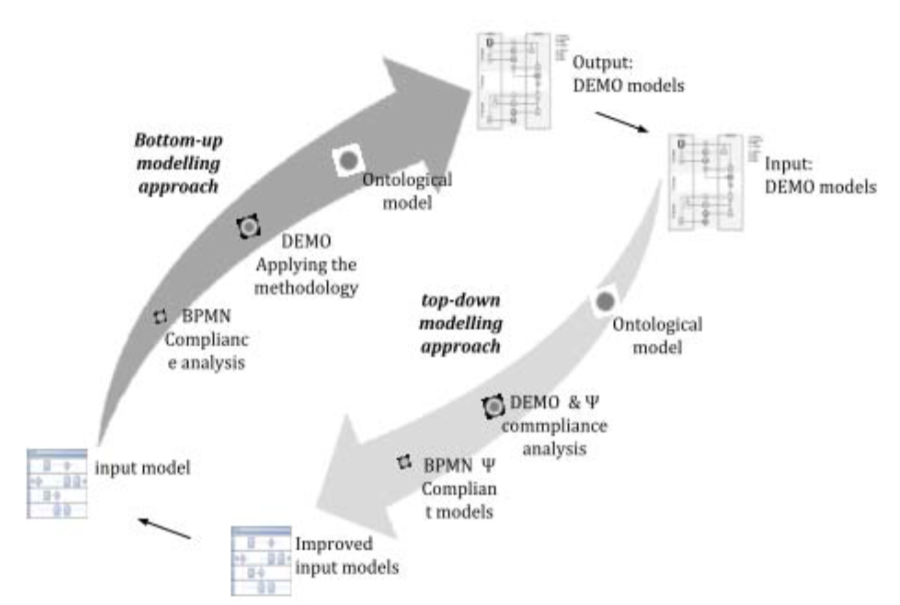
\includegraphics[width=\textwidth,height=\textheight,keepaspectratio]{obrazky/caetano-bpmn-demo-method}
\caption{Iterativní aplikace metody dle \cite{Caetano2011}}
\label{fig:caetano-bpmn-demo-method}
\end{figure}

\subsection{Rozšíření formálních základů BPMN pomocí Enterprise Ontology}

Práce \cite{VanNuffel2009} nazvaná \textit{Enhancing the Formal Foundations of BPMN by Enterprise Ontology} se na teoretické úrovni zabývá možností, jak využít Enterprise ontology jako ontologický základ pro vytváření BPMN modelů a argumentuje, že fundamentální koncepty BPMN jsou \uv{podobné} konceptům DEMO:

\begin{itemize}
\item Koncept \textit{aktivity} je \uv{podobný} konceptu výkonu (performance) nebo DEMO P-factu nebo určité komunikaci o tomto výkonu neboli DEMO C-factu.
\item Koncept \textit{plavecké dráhy} je \uv{podobný} konceptu actora (Actor-Iniciátor nebo Actor-Executor).
\end{itemize}

Na tomto základě a následnou důkladnou analýzou axiomů \ptheory autoři došli k 14 pozorováním. Jelikož jsou tato pozorování jedním ze základních stavebních kamenů metody navrhované v této práci budou zde uvedeny:

\begin{itemize}
\item Existují identifikovatelní \textit{actoři} plnící určité role, kde se actor vztahuje k roli a nikoli nutně k jedinci, který tuto roli fyzicky vykonává.
\item Existují identifikovatelné P-facty reprezentující nějaký \textit{úkon}.
\item Existují C-facty reprezentující \textit{komunikaci} o konkrétním úkonu, který má být vykonán.
\item Každý P-fact je vztažen pouze k jednomu unikátnímu C-factu a naopak.
\item Každý actor vyjma kořenového Actora-Iniciátora má jeden a pouze jeden vztah Actora-Exekutora k jednomu a pouze jednomu P-factu, ale může mít $0...n$ Actor-Iniciátor vztahů k jiným P-factům (potomkům).
\item Každý P-fact může být definován jako množina $0...n$ jeho potomků. %todo bullshit alert%
\item U každého rodičovského P-factu musí nejdřív dojít k dokončení (\textit{state} a \textit{accept}) P-factů, které jsou jeho potomky, dříve než může začít exekuce rodičovského P-factu.
\item Actor, který je exekutorem nějakého P-factu je zároveň iniciátorem každého P-factu, který je jeho potomkem.
\item Pouze iniciátor kořenového P-factu není iniciátorem žádného jiného P-factu.
\item U každého modelu existuje alespoň jeden P-fact, který je ve vztahu k actorovi, který je jen a pouze exekutorem tohoto P-factu.
\item Existuje množina osmi atributů (\textit{request}, \textit{promise}, etc.), které se unikátně vztahují ke konkrétnímu C-factu, který  popisuje aktuální stav komunikace ohledně úkonu (vytvoření P-factu).
\end{itemize}

Autoři ve své práci představují nástin dvou přístupů, jak využít DEMO a Enterprise Ontology pro vytváření či vylepšení BPMN modelů. Jedním z přístupů je analýza a doplnění existujících BPMN modelů na základě čtyř základních axiomů \ptheory v základu podobně jak bylo popsáno v sekci \ref{sec:analyza_proc_modelu_psi}. 

Pro tuto práci přínosnější je nástin druhé možnosti – vytváření nových BPMN modelů na formálním základě, který z DEMO a Enteprise Ontology vychází. Vytváření takového BPMN modelu začíná sběrem informací o organizaci, jejím chodu a funkci. Dalším krokem je aplikace \textit{distinkčního axiomu} a  vyřazení všech informací, které nejsou ontologické. Třetím krokem je pak ve zbylých informacích nalézt ontologické transakce a actory, kteří vystupují v rolích Actor-Iniciátor a Actor-Exekutor ve vztahu k těmto transakcím. Závěrečným krokem je pak vytvoření DEMO Actor-Transaction Diagramu, který zobrazuje vztah mezi transakcemi a actory. 

Výsledkem tohoto postupu tedy není BPMN model, ale kroky v něm nastíněné je nezbytné provést, aby bylo možné vytvořit BPMN model, který je \textit{konzistentní} a \textit{kompletní}. Metoda nastíněná v této práci právě na těchto krokech staví a posouvá je směrem ke skutečnému BPMN modelu.

\section{Mapování základních DEMO konceptů na BPMN primitiva}
\subsection{Výchozí předpoklady}
Důkladným studiem notace BPMN i metodologie DEMO bylo vypozorováno několik výchozích předpokladů, které navazují na pozorování dle \cite{VanNuffel2009}, která jsme uvedli v sekci \ref{sec:existujici_moznosti}.

\begin{itemize}
\item V notaci BPMN nenajdeme žádné transakce tak, jak je definuje DEMO. Ve verzi BPMN 2.0 sice konstrukt nazvaný transakce existuje, ale v tomto případě se jedná pouze o speciální druh elementů, který vyžaduje definici kompenzačních aktivit v případě, že je nutné transakci odvolat.
\item Neexistují tedy ani žádné pevně dané \textit{transakční kroky} a výsledný procesní model může mít takřka jakoukoliv strukturu.
\item Nejsou pevně specifikovány role účastníků (actorů) podnikového procesu.
\item Není pevně dáno, že každý proces musí obsahovat popis \uv{šťastných} i \uv{nešťastných} scénářů a ty \uv{nešťastné} se v praxi často nemodelují.
\item Není řečeno, které druhy aktivit se mají v modelu zachytit, a které jsou zbytné nebo příliš detailní.
\end{itemize}

\subsection{Základní pravidla používání notace BPMN} \label{sec:zakladni_pravidla}
V této sekci jsou vypsány základní pravidla, jak používat některé elementy z notace BPMN tak, aby jejich použití korespondovalo s vybranými koncepty z metodologie DEMO dle základu metody představené v této práci. Z metodologie DEMO byly vybrány zejména ty koncepty, které jsou součástí transakčního axiomu, který je pro vlastní tvorbu modelů podnikových procesů nejzásadnější a vyjádření tohoto axiomu pomocí korespondujících elementů BPMN by výrazně přispělo k možnosti vytvářet kvalitnější modely v této notaci tak, jak bylo popsáno v sekci \ref{sec:demo_bpmn_benefity}
\subsubsection{Vyjádření actorů}
\textit{Actor} je v DEMO definován jako kombinace \textit{odpovědnosti} a \textit{kompetence} a není nezbytně svázán s konkrétním jedincem, který ve výsledku aktivitu či transakci fyzicky provádí. Pokud chceme v BPMN transakce zobrazovat, musí se podařit v paletě elementů, které BPMN nabízí nalézt takové, pomocí kterých je možné aktory korektně vyjádřit. Vybraný element musí splňovat tyto předpoklady:

\begin{itemize}
\item Musí jasně určovat, které kroky transakčního axiomu (C-acty a P-acty) patří do pole zodpovědnosti daného actora.
\item Musí umožňovat \textit{komunikaci} s druhým actorem v transakci.
\item Musí umožňovat navazování dalších actorů a transakcí v \textit{transakčním stromu}.
\end{itemize}

Pro znázornění actora se nabízí využití BPMN elementu \textit{plavecká dráha (swimlane)}. BPMN nijak konkrétně nespecifikuje, jak plavecké dráhy využívat a nechává to tedy v rukou osoby, která model vytváří \cite{Silver2011}. Pro znázornění dvou actorů v transakci by pak sloužily dvě sousedící plavecké dráhy. Komunikace mezi nimi by pak probíhala především pomocí \textit{sekvenčních toků}.

Další možností, jak reprezentovat actora, je teoreticky použitím elementu \textit{bazén}, který by tak fungoval samostatně pro každého actora a jelikož standard notace BPMN 2.0 zakazuje, aby sekvenční toky překročily hranice bazénu, museli by actoři mezi sebou koordinovat kroky (C-acty, P-acty) pomocí zasílání zpráv. A právě zde tkví hlavní úskalí tohoto přístupu. V odborné literatuře (například \cite{Silver2011}) je obecně uváděno, že není dobrým přístupem modelovat aktivity v rámci jednoho procesu uvnitř více bazénů. Vznikají pak problémy v navazování posloupnosti aktivit na sebe, ale i s korektností výsledného BPMN modelu dle zásad DEMO neboť využití bazénů nám rozdělí transakci fakticky do dvou procesů, což přináší problémy, které budou popsány v sekci \ref{sec:tr_vzor_ulohy_zpravy}.

\subsubsection{Vyjádření C-actů a P-actů}
\textit{C-acty} a \textit{P-acty} jsou jednotlivé kroky v transakčním vzoru, které jsou prováděny v definovaném pořadí a jsou v transakci vždy přítomny, i když jsou někdy prováděny \textit{mlčky}. Pro vyjádření C-actů a P-actů navrhovaná metoda využívá BPMN element \textit{úloha (Task)}, který je dále nedělitelným typem \textit{aktivity}. Úlohy mohou být dále rozlčleněny na ty, které provádí člověk, které systém nebo nějaký stroj atp. Pro účely modelování popsané v této práci se nejlépe hodí abstraktní úlohy, které jsou bez označení. 

V předchozím odstavci bylo zmíněno, že některé transakční kroky mohou být prováděny \textit{mlčky}. To znamená, že ve skutečnosti neexistuje žádná aktivita, která by daný C-act prováděla, nicméně i provedení C-actu \textit{mlčky} se dle metodologie DEMO počítá jako faktické provedení C-actu. \cite{Dietz2006}

\subsubsection{Vyjádření C-factů} \label{sec:vyjadreni_cfactu}
\textit{C-fact} neboli \textit{coordination fact} je výsledkem provedení C-actu. Je tedy přímo navázán na C-act, který jej \uv{vytváří}. V BPMN lze C-fact vyjádřit třemi způsoby:

\begin{enumerate}
\item C-fact v modelu není explicitně vyjádřen. Jeho existence je zajištěna implicitně pomocí \textit{sekvenčních toků} vycházejících z \textit{úloh}, které reprezentují C-act.
\item C-fact je vyjádřen pomocí \textit{signálu}. Důvod pro použití elementu signál je ten, že druhý actor by měl být o vzniku C-factu (respektive změně \textit{C-worldu}) informován, což způsob představený v bodě 1 nezaručuje.
\item C-fact je vyjádřen pomocí \textit{zprávy}, kterou zašle actor, který příslušný C-act vykonal druhému actorovi.
\end{enumerate}

V \cite{Dietz2006} se uvádí, že v DEMO modelech je C-fact zakreslen mezi elementy, které reprezentují role actorů, což znamená, že C-fact, existuje v jejich společném \textit{mezisvětě} neboli oba actoři mohou o vzniku C-factu vědět. Z toho vyplývá, že pro reprezentaci C-factu je nejvhodnější některý ze způsobů uvedených v bodech 2 nebo 3.

\subsubsection{Vyjádření P-factů}
Podobně jako C-fact je i \textit{P-fact} výsledkem provedení konkrétního P-actu. V transakci se objevuje pouze jednou a zjednodušeně lze říci, že je \uv{výsledkem} celé transakce. P-fact může být hmotné povahy (např. upečení pizzy), ale i nehmotné (např. rozhodnutí poroty). Metoda, která je nastíněna v této práci, P-fact v modelu BPMN explicitně neuvádí. Důvody pro toto rozhodnutí jsou následující:

\begin{itemize}
\item Korespondující P-act (vyjádřený \textit{úlohou}) nazvaný \textit{Execute} a \textit{sekvenční tok} z něj vycházející už sami o sobě vyjadřují vznik P-factu.
\item Actor-Iniciátor je o vzniku P-factu informován ve chvíli, kdy je mu předložen pomocí C-actu \textit{state}, který dle transakčního axiomu nastane vždy.
\item Ve standardním i základním transakčním vzoru v metodologii DEMO je P-act i P-fact uváděn pouze v rámci agendy patřící Actorovi-Exekutorovi.
\end{itemize}

\subsubsection{Vyjádření Agendy}

\begin{quote}
Slovo \uv{agenda} vyjadřuje \uv{co musí být uděláno} neboli agenda je \uv{úkol k vyřešení}. \cite{Dietz2006}
\footnote{The word “agendum” is the singular form of the (plural) Latin word “agenda”. It means: what has to be done. In other words, an agendum is a to-do item. \cite{Dietz2006}}
\end{quote}

V metodologii DEMO nejednají Actoři náhodně, ale každý jejich krok je striktně definován pomocí \textit{action rules} v DEMO Action Modelu. Například je jasně řečeno  za jakých okolností se vytvoření P-factu přislíbí (\textit{promise}) a kdy je nutné \textit{request} odmítnout. \textit{Agenda} dle DEMO je tvořena čtveřicí parametrů:

\begin{itemize}
\item \textit{C-fact}, který má být vykonán.
\item \textit{P-fact}, kterého se C-fact týká,
\item \textit{Čas} vztahující se k provedení P-factu.
\item \textit{Čas}, kdy by měl být C-fact vykonán. %bullshit alert%
\end{itemize}

Jelikož návrh metody, který tato práce popisuje, pracuje pouze s existujícími BPMN elementy, není v tuto chvíli možné kompletní Agendu pomocí nich vyjádřit. Řešením by bylo buď vytvořit vlastní doplňující model podobný DEMO Action Modelu nebo přímo DEMO Action Model. Dalším výzkumem je nutné ověřit, zda je vytvoření takové vrstvy nutné a případně takovou vrstvu vytvořit tak, aby byla připravena pro implementaci v softwarovém nástroji, který by tak umožnil simulaci modelovaného procesu.

Metodologie navrhovaná v této práci si vystačí s částečným zobrazením agendy přímo v BPMN modelu, kterého je docíleno pomocí \textit{plavecké dráhy} (případně \textit{bazénu}), \textit{sekvenčního toku} a \textit{časového hlediska}. Jinými slovy díky plavecké dráze nebo bazénu, který obsahuje elementy, jež spadají do kompetence a odpovědnosti actora, kterému je plavecká dráha nebo bazén příslušná a díky sekvenčnímu toku, který určuje pořadí provádění jednotlivých úloh daný actor v každém momentě v čase ví, kterou úlohu má provést. Pravidla pro vyhodnocení, zda přijmout \textit{request} nebo \textit{state} pro zjednodušení opomíjíme.

\section{Vyjádření transakčního vzoru v BPMN} \label{sec:vyjadreni_trans_vzor}
Pro metodologii, která je nastíněna v této práci je transakční vzor dle transakčního axiomu DEMO tím nejdůležitějším stavebním kamenem. Dává totiž řád a jasnou strukturu tomu, jak popsat podnikový proces, který je dle metodologie DEMO jen uspořádanou strukturou na sebe navázaných transakcí – \textit{transakčním stromem}.

Vyjádření transakčního vzoru pomocí elementů z notace BPMN je tak zcela zásadní pro to, aby mohl být naplněn účel nově vznikající metody, kterým je přispět k vytváření BPMN modelů, které budou \textit{kompletní} a \textit{jednoznačné}. Jak bylo popsáno v sekci \ref{sec:zakladni_pravidla}, vyjádření jednotlivých komponent transakčního vzoru je možné provést pomocí různých elementů a v této sekci jsou tyto různé přístupy rozebrány do většího detailu. 

\subsection{Vyjádření pomocí \textit{úloh}} \label{sec:vyjadreni_ulohy}
Prvním a nejjednoduším přístupem je vyjádřit transakční vzor čistě pomocí \textit{úloh} a \textit{sekvenčních toků}. Úlohy jsou použity pro vyjádření \textit{C-actů} a \textit{P-actů}. Sekvenční tok je použit ve více významech:

\begin{itemize}
\item jednak pro určení \textit{pořadí} provádění jednotlivých C-actů,
\item jednak pro zadávání C-factů do \textit{agendy} druhému actorovi,
\item jednak sekvenční tok vycházející z každé úlohy reprezentující C-act reprezentuje úspěšný \textit{vznik korespondujícího C-factu}.
\end{itemize}

Na obrázku \ref{fig:Zk_trans_ulohy} je zobrazen \textit{základní transakční vzor} pomocí úloh. \textit{Bazén} slouží pro zastřešení celé transakce a \textit{plavecké dráhy} oddělují agendy obou zúčastněných actorů (Iniciátora a Exektuora). Základní transakční vzor bere v potaz pouze \uv{šťastné scénáře}, takže transakce vždy skončí ve stavu \textit{T1 Accepted}. Všechny C-facty, ze kterých transakce již nikam dál nepokračuje jsou vyjádřeny BPMN elementem \textit{konečná událost (End event)}.

Obrázek \ref{fig:St_trans_ulohy} zobrazuje \textit{standardní transakční vzor}, tedy kompletní transakci včetně všech \uv{nešťastných scénářů (unhappy paths)}. Oproti základnímu transakčnímu vzoru zde přibyly čtyři \textit{brány} označující místo, kde actor musí rozhodnout, jak s agendou naloží. Rozhodnutí je exkluzivní, tudíž je použita \textit{exkluzivní brána XOR}.

V tomto zobrazení nejsou zobrazeny žádné C-facty, což je z hlediska DEMO problematické. Ačkoliv jejich vznik vyjadřuje sekvenční tok vycházející z C-actu, C-fact není explicitně vyobrazen a druhý actor o něm nemusí vědět, protože v modelu není žádná komunikace zobrazena. Dle \cite{Dietz2006} však oba Actoři mají mít umožněno vědět o vzniku C-factu.

\begin{figure}[H]\centering
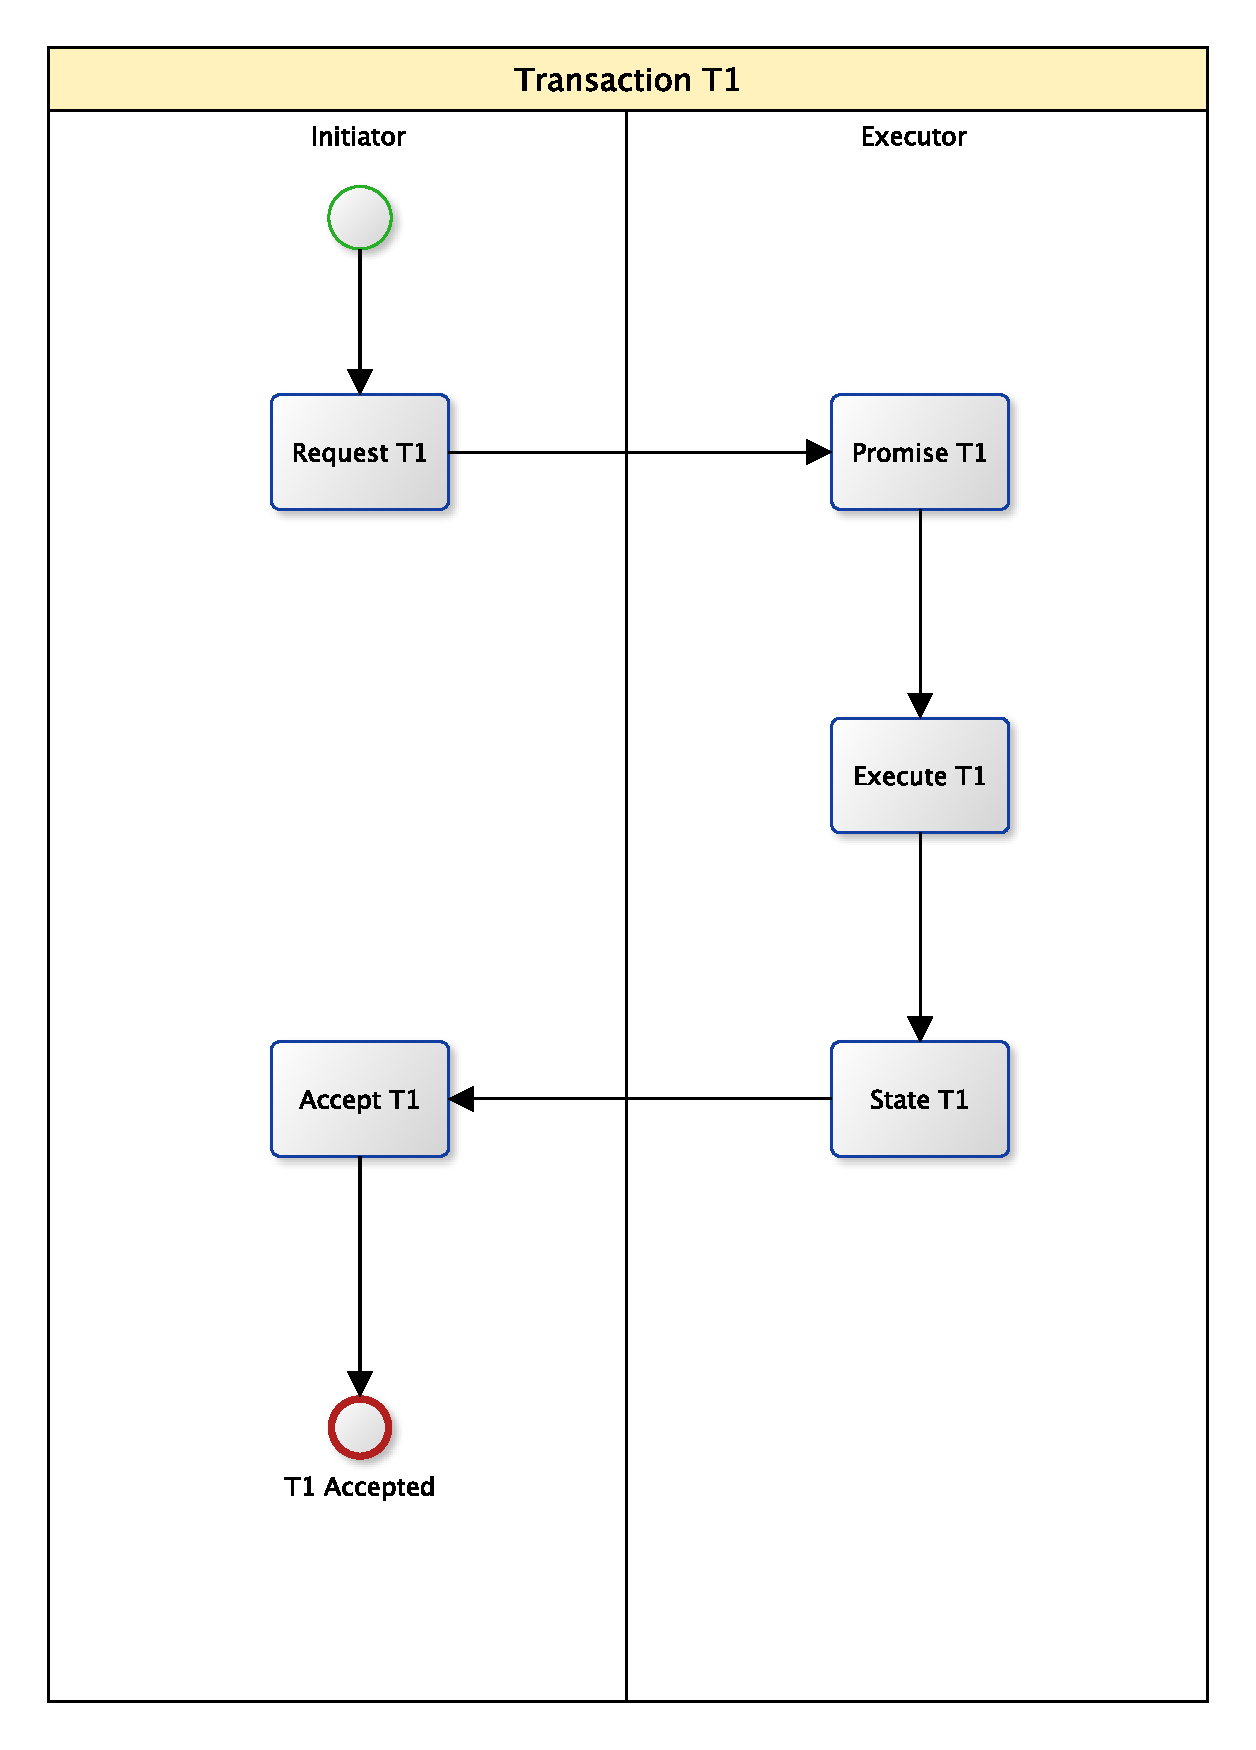
\includegraphics[width=1.0\textwidth]{obrazky/transaction-basic-tasks}
\caption{Základní transakční vzor pomocí Úloh}
\label{fig:Zk_trans_ulohy}
\end{figure}

\begin{figure}[H]\centering
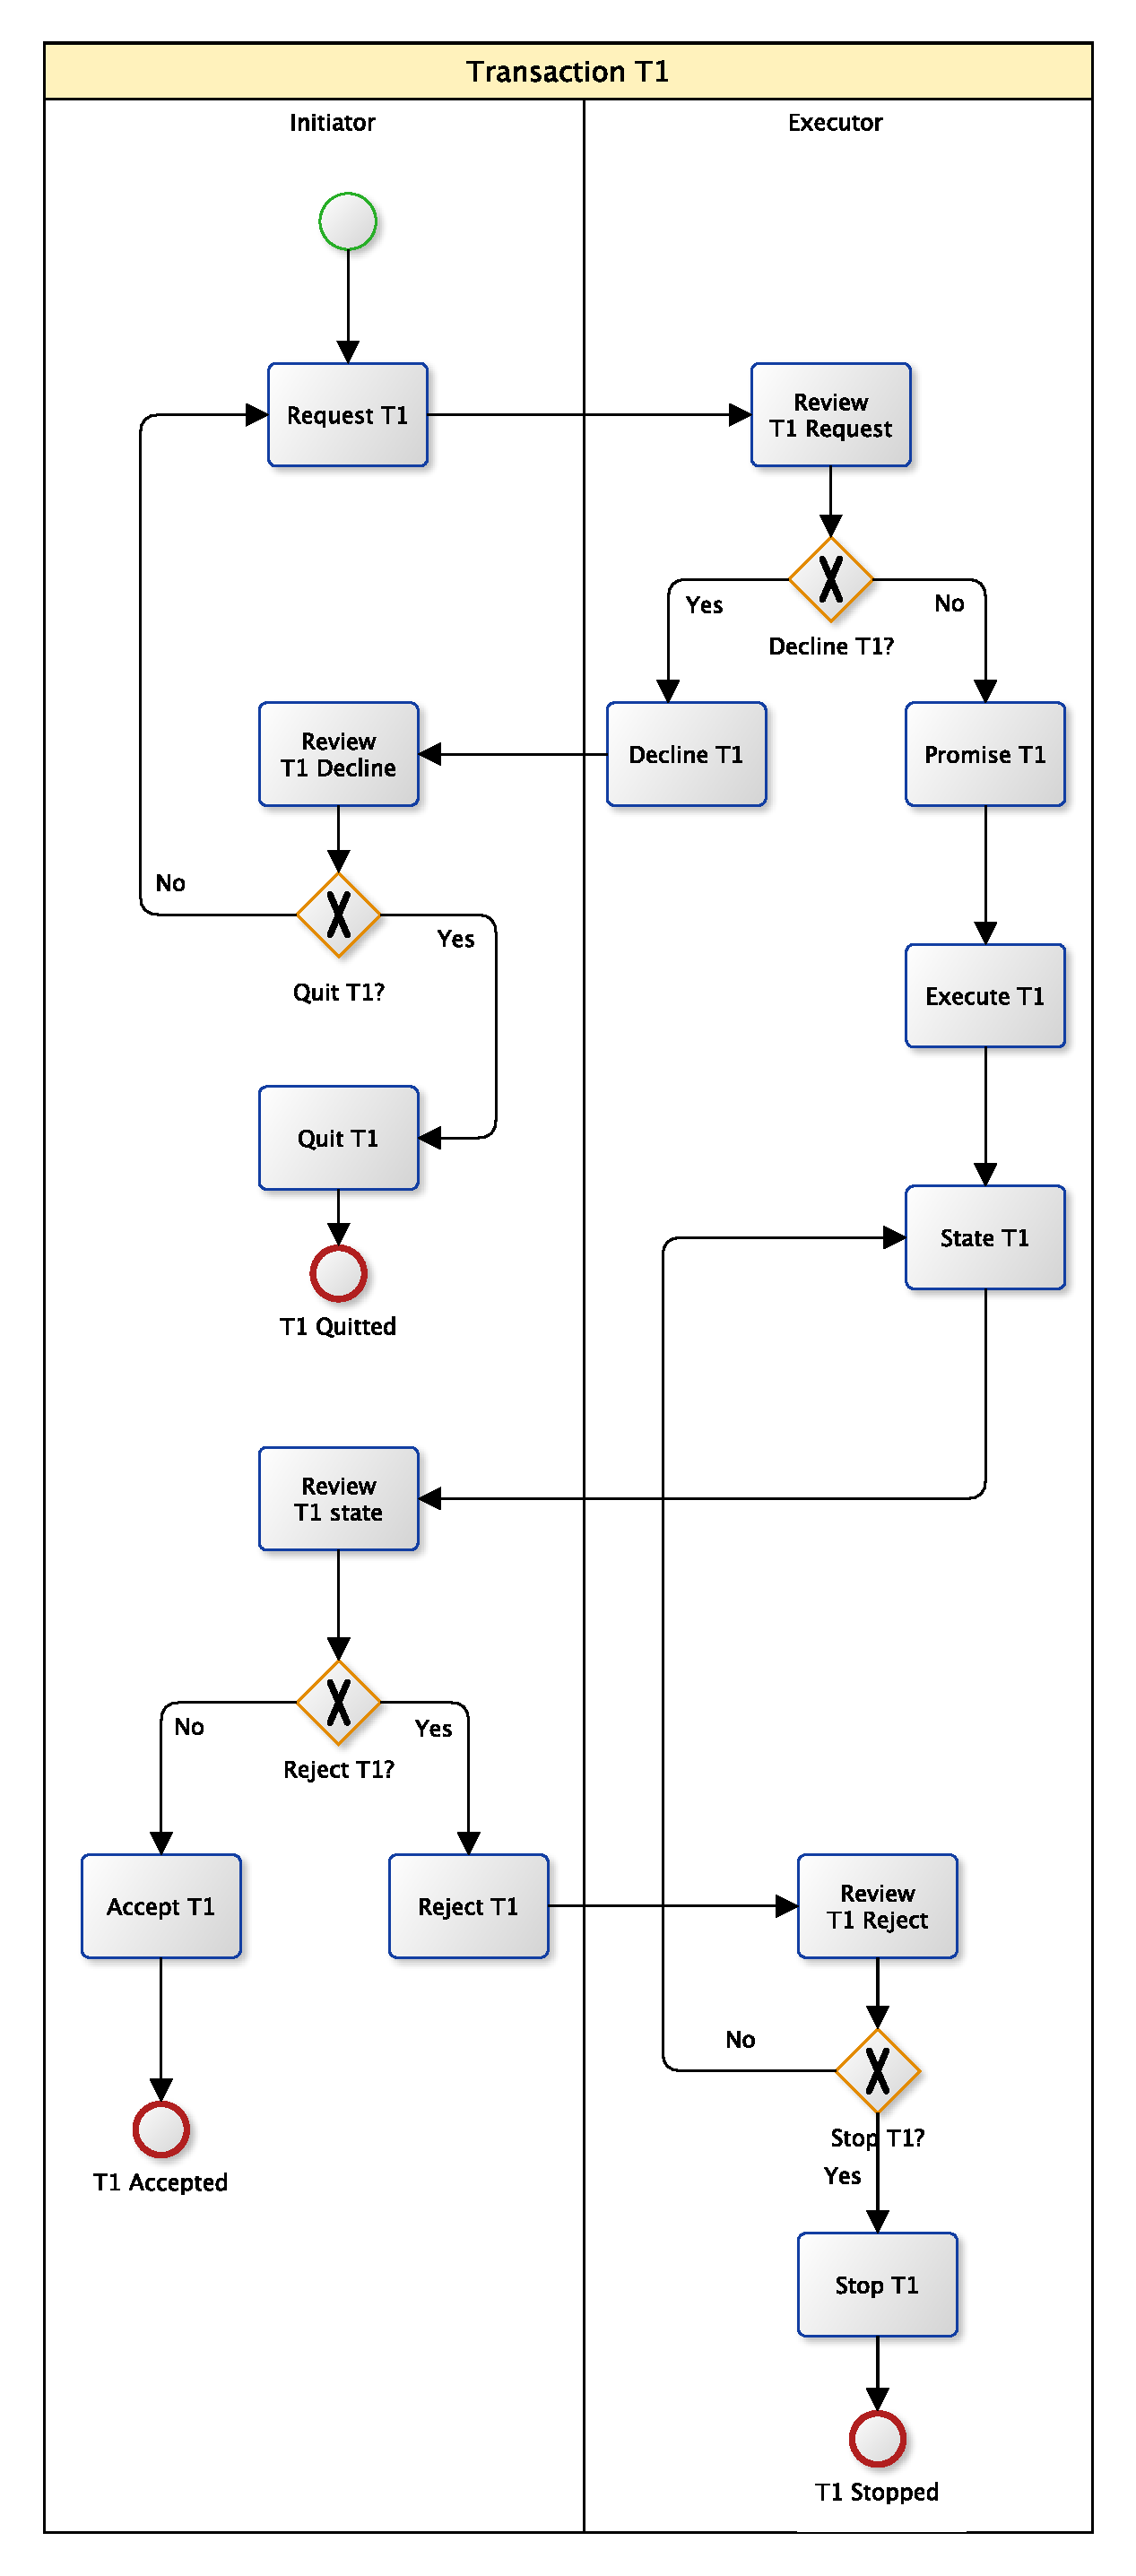
\includegraphics[width=\textwidth,height=\textheight,keepaspectratio]{obrazky/transaction-standard-tasks}
\caption{Standardní transakční vzor pomocí Úloh}
\label{fig:St_trans_ulohy}
\end{figure}

\subsection{Vyjádření pomocí \textit{úloh} a \textit{signálů}} \label{sec:tr_vzor_ulohy_signaly}

Další možností, jak transakční vzor zobrazit, je využití \textit{úloh} a \textit{signálů}. Narozdíl od způsobu popsaného v sekci \ref{sec:vyjadreni_ulohy} slouží \textit{sekvenční toky} v tomto případě  pouze k vyjádření pořadí, ve kterém jsou C-acty prováděny a pro předávání agendy mezi actory. O reprezentaci vzniklého C-factu se zde však stará BPMN element \textit{signál}, což poskytuje dvě velké výhody. Jednak je díky tomu C-fact v modelu vizuálně zastoupen, takže se výsledný model více blíží transakčnímu vzoru tak, jak ho definuje DEMO a jednak BPMN element signál e dle specifikace \cite{Omg2011} i \cite{Silver2011} možné použít ke komunikaci uvnitř procesu, respektive k odeslání neadresné zprávy komukoliv, kdo je připraven jí naslouchat. Toto mnohem přesněji vyhovuje popisu společného \textit{mezisvěta}, který jsme uvedli v sekci \label{sec:vyjadreni_cfactu}.

Pro reprezentaci actorů jsou v tomto případě opět použity \textit{plavecké dráhy} uvnitř \textit{bazénu}, který zastřešuje celou transakci. C-facty, ve kterých transakce končí jsou i v tomto případě vyjádřeny pomocí BPMN elementu \textit{konečná událost}.

Na obrázku \ref{fig:Zk_trans_ulohy_signaly} vidíme \textit{základní transakční vzor} pomocí úloh a signálů. Lze vidět, že po provedení C-actu \textit{Request T1} se sekvenční tok přesouvá do signálu \textit{T1 Requested}, který vyjadřuje vzniklý C-fact. Předpokládáme, že Actor-Executor tomuto Signálu naslouchá a může tak provést C-act \textit{Promise T1}.

Obrázek \ref{fig:St_trans_ulohy_signaly} zobrazuje \textit{standardní transakční vzor} vyjádřený úlohami a signály.

\begin{figure}[H]\centering
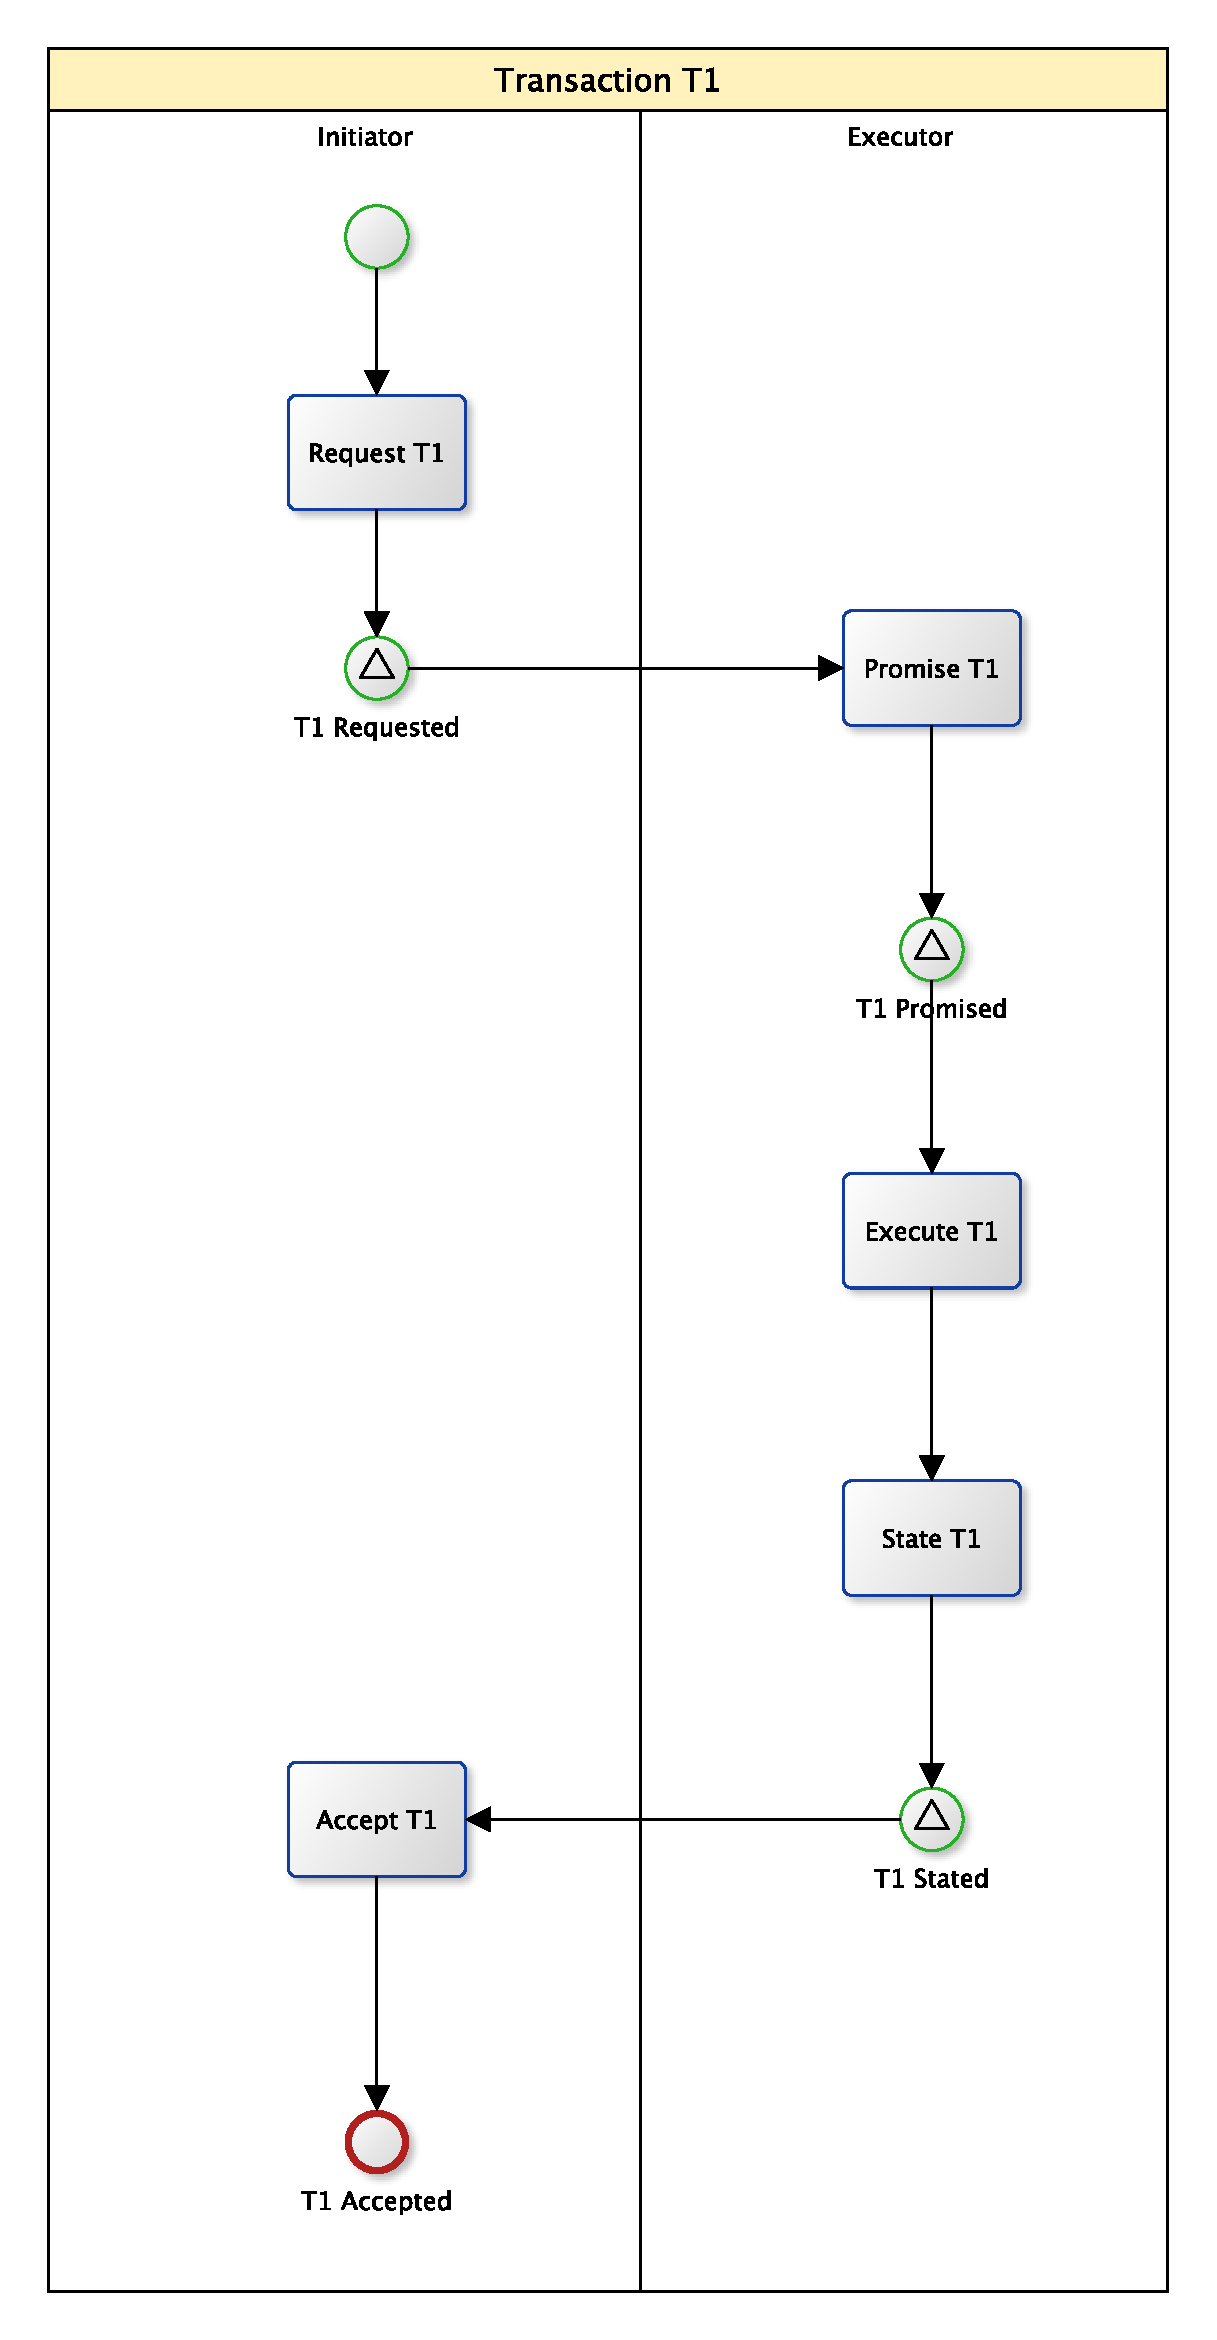
\includegraphics[width=\textwidth,height=\textheight,keepaspectratio]{obrazky/transaction-basic-signals}
\caption{Základní transakční vzor pomocí Úloh a Signálů}
\label{fig:Zk_trans_ulohy_signaly}
\end{figure}

\begin{figure}[H]\centering
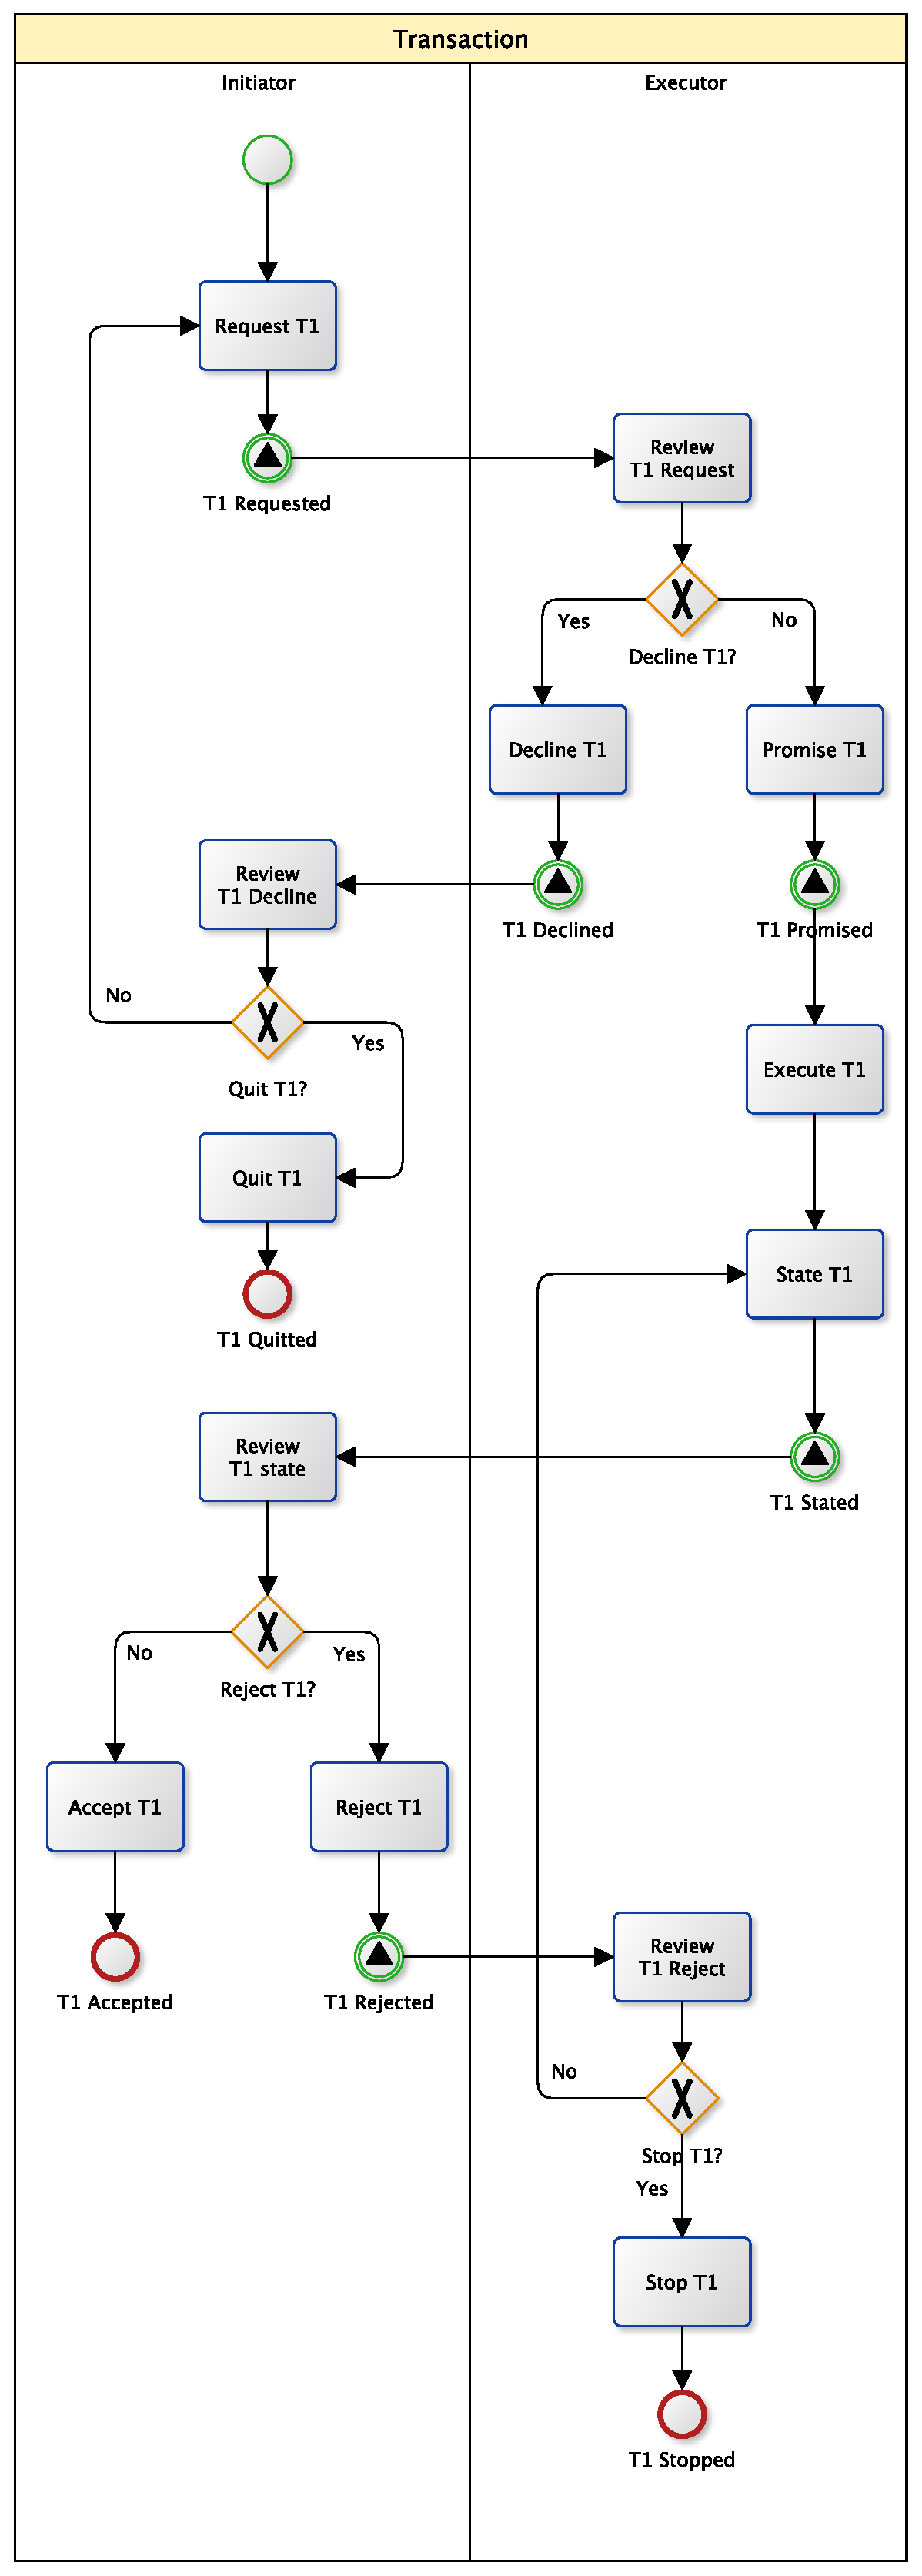
\includegraphics[width=\textwidth,height=\textheight,keepaspectratio]{obrazky/transaction-standard-signals}
\caption{Standardní transakční vzor pomocí Úloh a Signálů}
\label{fig:St_trans_ulohy_signaly}
\end{figure}

\subsection{Vyjádření pomocí Úloh a Zpráv} \label{sec:tr_vzor_ulohy_zpravy}
Jiným přístupem k vyjádření transakčního vzoru je využít ke komunikaci mezi actory BPMN element \textit{zpráva}. Jelikož specifikace BPMN předepisuje, že zpráva může být použita pouze ke komunikaci mezi \textit{bazény}, musí být v tomto případě pro každého actora vyhrazen zvláštní bazén. Na obrázku \ref{fig:Zk_trans_ulohy_zpravy} lze vidět \textit{základní transakční vzor} vyjádřený právě tímto způsobem.

Předávání agendy v tomto případě probíhá pomocí zaslání zprávy a  \textit{průběžné události (Intermediate event)}. Jakmile \textit{Actor-Iniciátor} provede C-act \textit{Request T1}, vyšle zprávu reprezentující C-fact, kterou přijme \textit{Actor-Exekutor} na druhé straně pomocí \textit{počáteční události} typu \textit{catch (Message)}, čímž vznikne nová instance procesu na straně Exekutora. O každém provedeném C-actu je pak druhý actor informován pomocí zprávy. 

V případě základního transakčního vzoru se většina problematických míst tohoto přístupu neprojevuje. K diskusi je však rozdělení actorů do dvou bazénů, které v podstatě znamená rozdělení transakce na dva podprocesy, jeden na straně Iniciátora a jeden na straně Exekutora. Toto je poměrně výrazné odchýlení od transakčního axiomu tak, jak ho definuje DEMO a přináší komplikace, které se projeví v případě \textit{standardního transakčního vzoru}.

Ve standardním transakčním vzoru totiž existují místa, která při maximální snaze o dodržení standardního transakčního vzoru z DEMO mohou vyústit v \textit{deadlock}. Jedná se o případy, kdy se actor rozhodne zamítnout výsledek C-actu \textit{request} nebo \textit{state}. V takovém případě totiž musí actor odpovědný za C-act rozhodnout, zda transakci zastavit nebo se pokusit o C-act znovu. Transakční vzor dle DEMO, ale nepočítá s tím, že by transakce byla rozdělena mezi dva procesy a že by měl existovat mechanismus, jak o tomto rozhodnutí informovat druhého actora. Řešením je v tomto případě přidat do transakčního vzoru mezistavové zprávy.

V případě, že bychom nepoužili mezistavové zprávy, nastal by problém hned v případě, že by se Actor-Exekutor rozhodl pro \textit{Decline T1}. V takovém případě Exekutor vyšle zprávu Actoru-Iniciátorovi a ten může buď transakci zastavit použitím \textit{Quit T1} nebo poslat \textit{Request T1} znovu. Jenže sekvenční tok v procesu na straně Exekutora je stále v situaci \textit{Decline T1} a bez mezistavové zprávy (neboli zprávy o rozhodnutí jak se Iniciátor rozhodl naložit s \textit{T1 Declined}) nemůže dále pokračovat. Částečným řešením, které můžeme vidět na obrázku \ref{fig:St_trans_ulohy_zpravy}, by v tomto případě mohlo být použít na tomto místě koncový stav \textit{T1 Declined} a instanci procesu u Exekutora ukončit. V případě, že by se Iniciátor rozhodl transakci neukončit a poslal \textit{request} znovu, vznikla by nová instanci procesu na straně Exekutora.

Větší problém však nastane v případě, kdy by se Iniciátor po obdržení \textit{T1 State} rozhodl tento \textit{state} odmítnout a provést \textit{Reject T1}. Exekutor by následně obdržel zprávu o \textit{rejectu} a musel by rozhodnout, zda transakci zastavit provedením \textit{Stop T1} nebo provést \textit{State T1} znovu. Jenže bez mezistavových zpráv se Iniciátor nemá šanci dozvědět výsledek tohoto rozhodnutí Exekutora. Řešení popsané v předchozím odstavci zde nebude fungovat, protože pokud by se Exekutor rozhodl provést znovu \textit{State T1}, proces na straně Iniciátora by již byl ukončen. Jediným řešením jsou tedy mezistavové zprávy, které informují druhého actora o rozhodnutích v případě, kdy by mohlo dojít k deadlocku. Toto řešení lze vidět na obrázku \ref{fig:St_trans_ulohy_zpravy_mezistav}. Jakmile nastane \textit{Decline T1} proces na straně Exekutora se přesune do\textit{ průběžné události (Multiple)} a čeká na příchod mezistavové zprávy od Iniciátora, jestli se rozhodl transakci ukončit nebo pošle \textit{request} znovu. Na základě toho buď proces ukončí nebo ho přesune na začátek a bude čekat na \textit{request} od Iniciátora. Analogicky je pak mezistavových zpráv využito v případě \textit{state}.

Využití mezistavových zpráv je však výrazným odchýlením od transakčního axiomu, protože tyto zprávy fakticky přidávají další komunikaci, se kterou transakční axiom nepočítá. Z tohoto důvodu je tento způsob pro vyjádření transakčního axiomu nevhodný. 

\begin{figure}[H]\centering
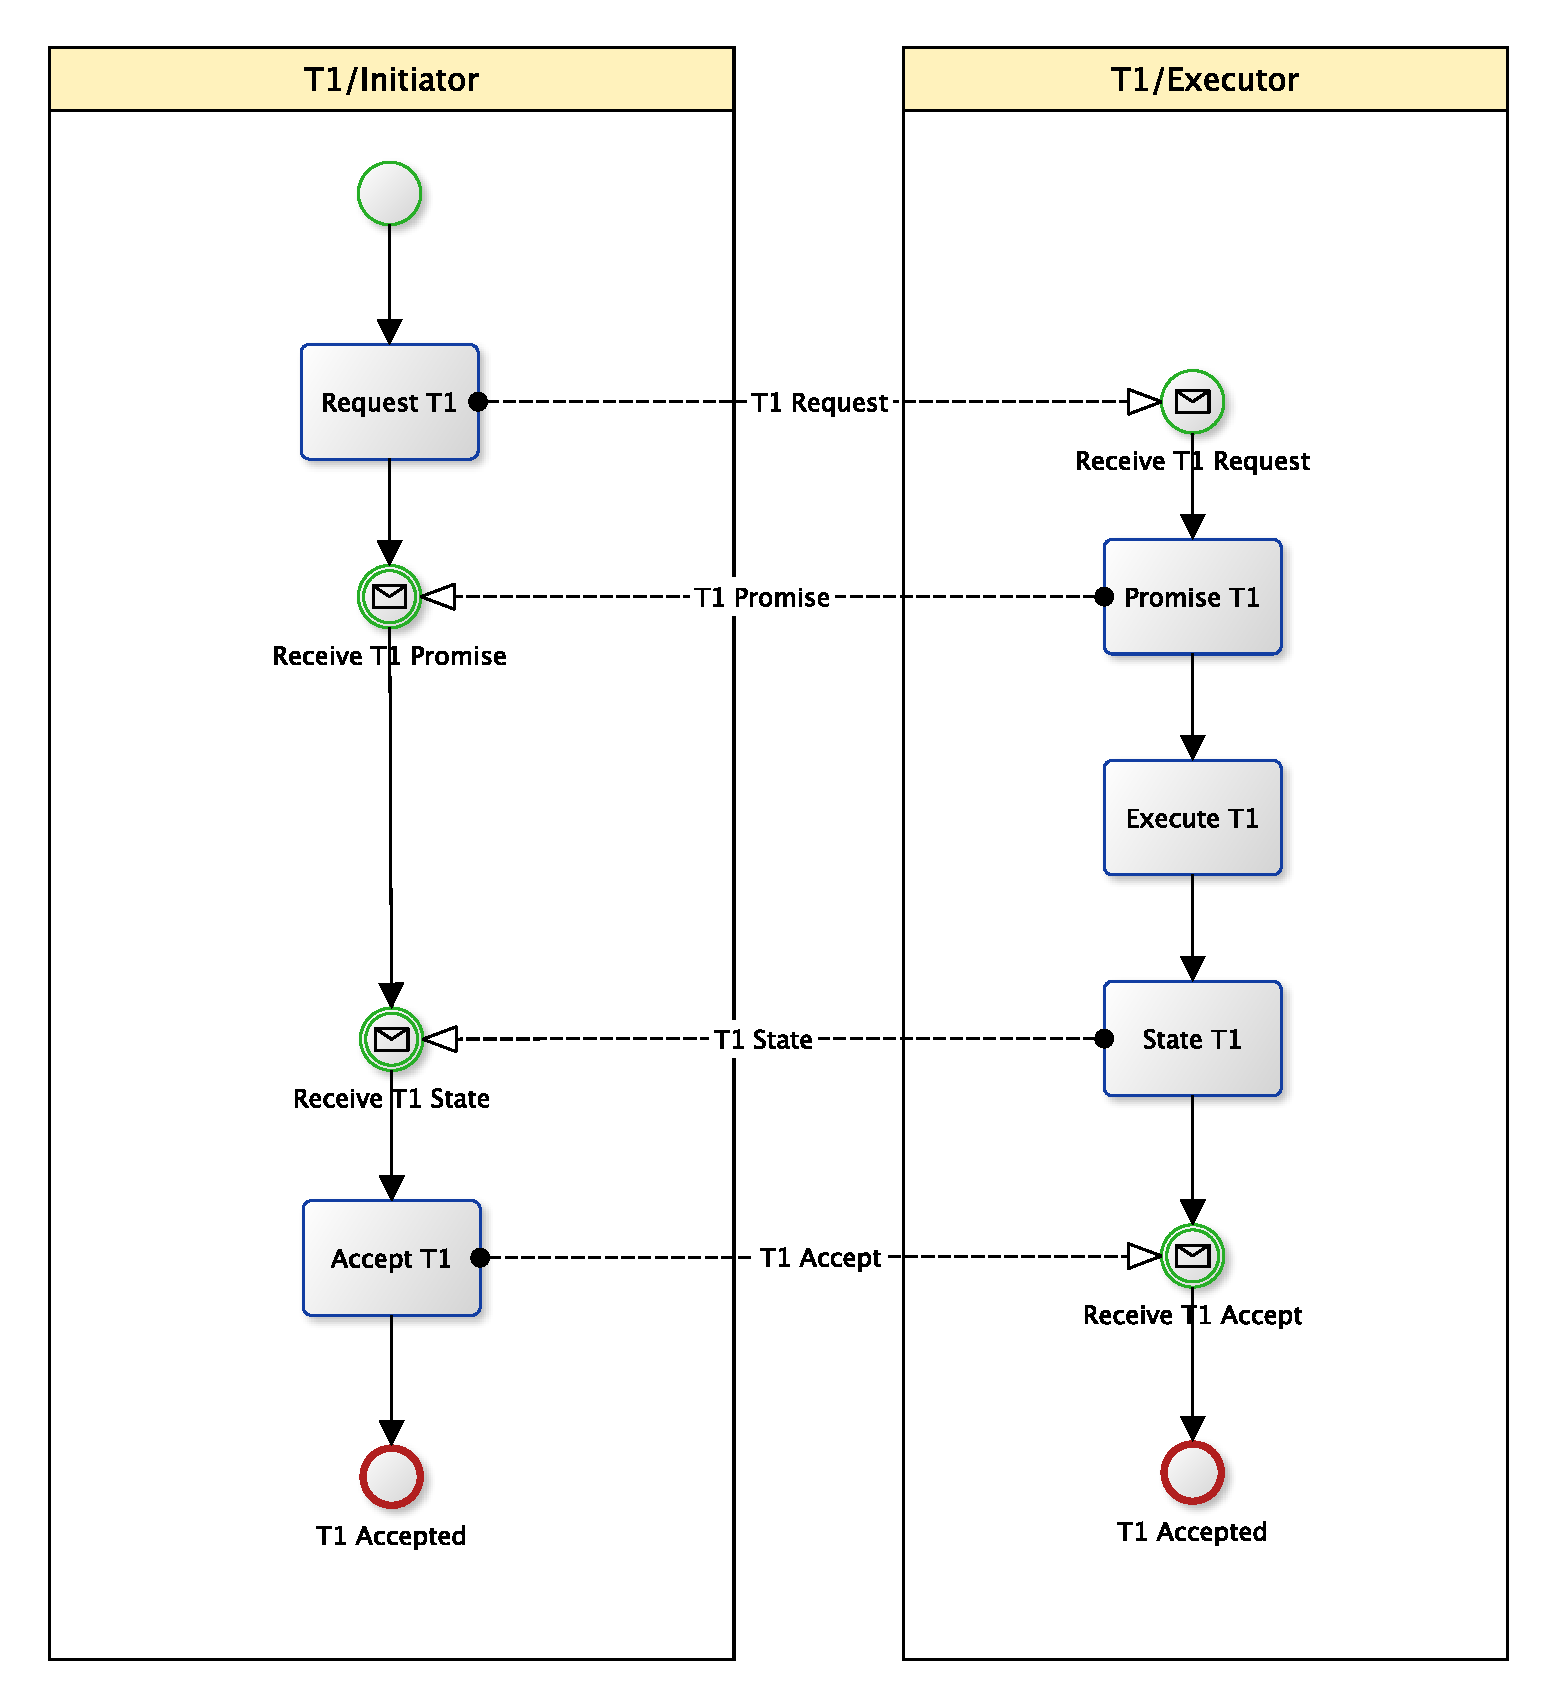
\includegraphics[width=\textwidth,height=\textheight,keepaspectratio]{obrazky/transaction-basic-messages}
\caption{Základní transakční vzor pomocí \textit{úloh} a \textit{zpráv}}
\label{fig:Zk_trans_ulohy_zpravy}
\end{figure}

\begin{figure}[H]\centering
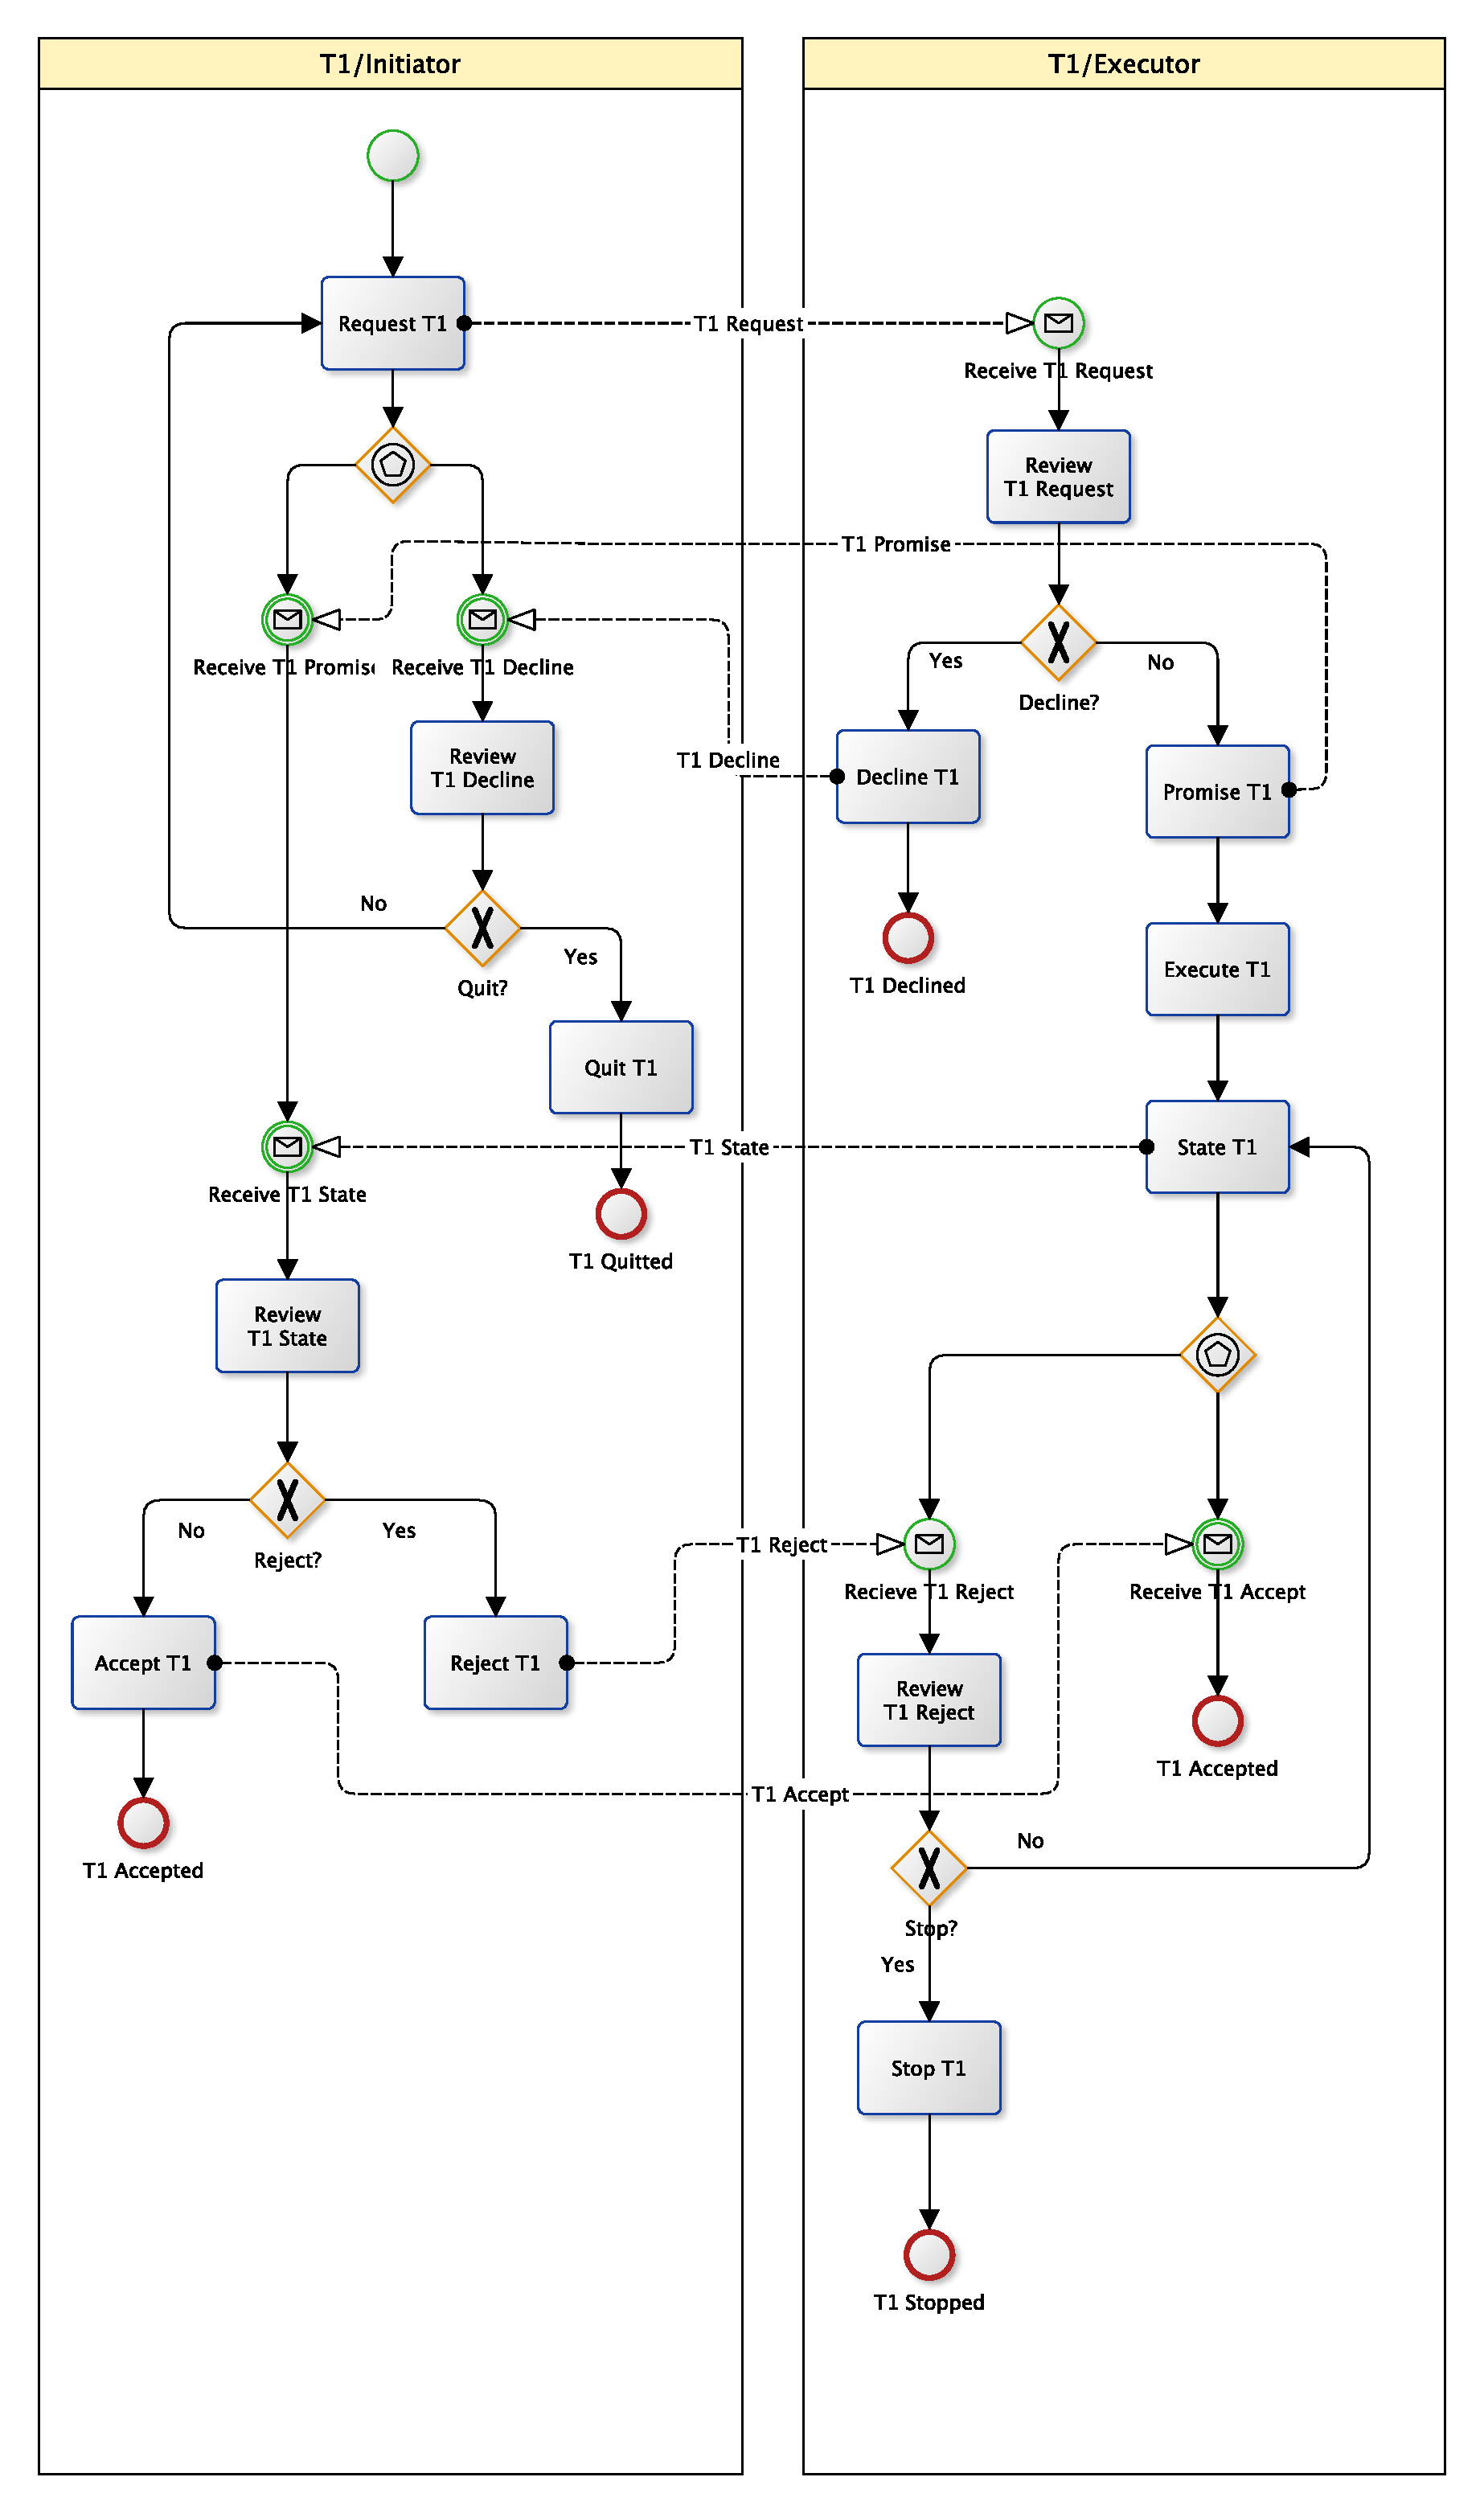
\includegraphics[width=\textwidth,height=\textheight,keepaspectratio]{obrazky/transaction-standard-messages-1}
\caption{Standardní transakční vzor pomocí \textit{úloh} a \textit{zpráv}}
\label{fig:St_trans_ulohy_zpravy}
\end{figure}

\begin{figure}[H]\centering
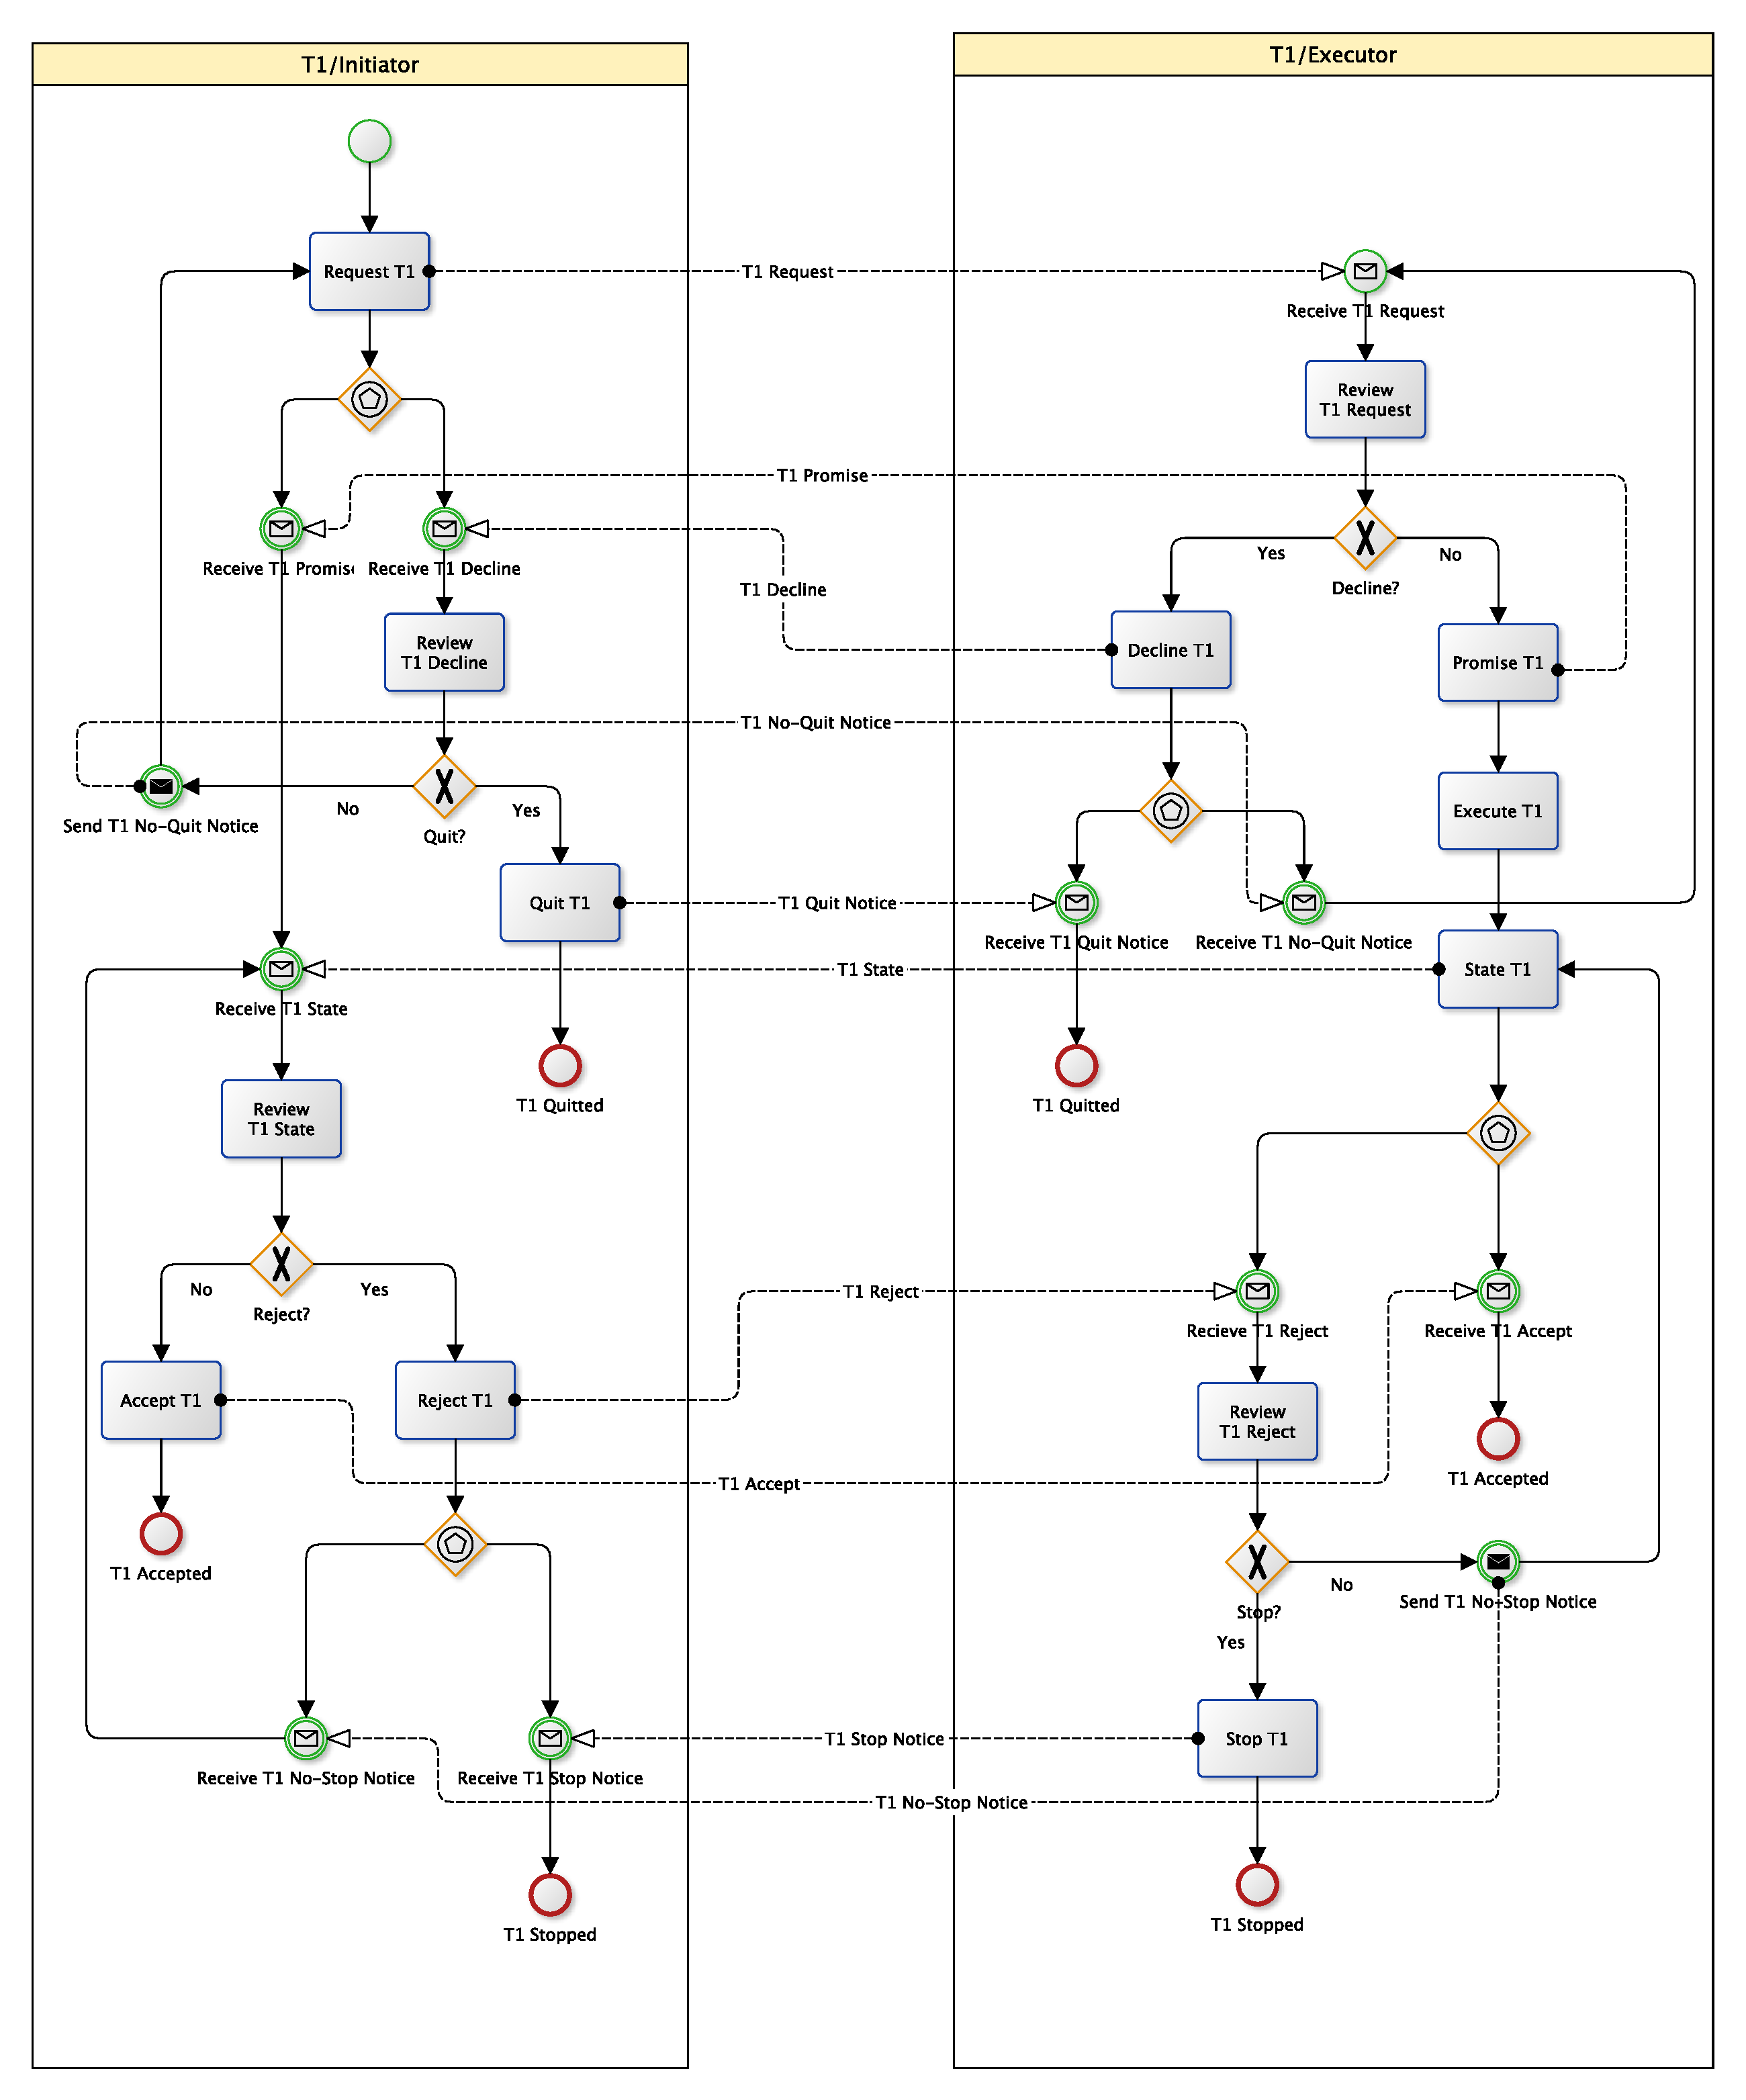
\includegraphics[width=\textwidth,height=\textheight,keepaspectratio]{obrazky/transaction-standard-messages}
\caption{Standardní transakční vzor pomocí \textit{úloh} a \textit{zpráv} (včetně mezistavových zpráv)}
\label{fig:St_trans_ulohy_zpravy_mezistav}
\end{figure}

\section{Návrh metody pro vytváření BPMN modelů dle zásad DEMO}
V této sekci je popsána metoda pro vytváření BPMN dle zásad DEMO. Představená metoda je navržena pro vytváření zcela nových modelů, nikoli k analýze a doplnění již existujících BPMN modelů. Cílem této metody je umožnit popisovat průběh podnikových procesů v oblíbené notaci BPMN a zároveň zajistit, aby výsledný model byl \textit{kompletní} a \textit{konzistentní}.

\subsection{Předpoklady}
Aby bylo možné implementovat tuto metodu v praxi, je nezbytné, aby odpovědní pracovníci byli vybaveni následujícími teoretickými znalostmi, které vycházejí z \ptheory, Enteprise ontology a metodologie DEMO.

\begin{itemize}
\item Znalost \textit{operačního axiomu} a schopnost rozlišit komunikační acty od produkčních.
\item Znalost \textit{transakčního axiomu}, \textit{základního i standardního transakčního vzoru} včetně všech jeho kroků (C-actů, C-factů, P-actů, P-factů).
\item Znalost a schopnost vytvořit DEMO Actor-Transaction Diagram (ATD) a DEMO Process Structure Diagram (PSD).
\item Znalost notace BPMN včetně elementů, které oblíbená publikace \cite{Silver2011} označuje jako Level 2.
\item Znalost a schopnost aplikovat \textit{kompoziční axiom}, tedy umět identifikovat jak jsou na sebe transakce navázané.
\end{itemize}

\subsection{Krok 1: Získání textového popisu procesu}
Při vytváření modelu určitého podnikového procesu je obvyklým prvním krokem získání informací od osob, které se tohoto procesu účastní nebo mu dobře rozumí. Může se jednat o výkonné i vedoucí pracovníky a obvykle je užitečné posbírat více pohledů na jeden konkrétní proces a následně diskutovat nesrovnalosti, které mohou vzniknout.

Díky tomu, že sběr informací provádějí pracovníci se znalostí transakčního axiomu i transakčních vzorů, mohou se cíleně zeptat na jednotlivé jeho kroky. Tedy zjistit, jak probíhá \textit{request}, jak \textit{state}, jak \textit{accept} a podobně. Na konci by tedy měl vzniknout textový popis procesu s maximem relevantních informací pro další postup.

\subsection{Krok 2: Aplikace distinkčního axiomu}
Nyní jsme schopni na vzniklý textový popis procesu, chodu organizace či její složky aplikovat tzv. \textit{Performa-Informa-Forma analýzu}, což není nic jiného než praktická aplikace \textit{distinkčního axiomu}, který je popsán v sekci \ref{sec:distinction_axiom}. Použijeme stejný postup jako v \cite{Dietz2006} a v textovém popisu označíme Performa aktivity červeně, Informa zeleně a Forma modře. Je naprosto přirozené, že u některých aktivit v textu bude problematické určit o jaký druh se jedná. S tím, jak budeme provádět další kroky dojdeme i k většímu porozumění celému procesu a je možné rozhodnutí přehodnotit. Výsledkem této části tedy je textový popis procesu s identifikovanými a vizuálně označenými Performa, Informa a Forma aktivitami.

\subsection{Krok 3: Aplikace operačního axiomu} \label{sec:st3_opax}
V tomto kroku budeme pracovat pouze s aktivitami, které jsme v Kroku 2 označili jako Performa (červeně). Úkolem je rozlišit, zda se jedná o C-act, C-fact, P-act nebo P-fact a dále k nim identifikovat příslušné actory tak jak předepisuje \textit{operační axiom} popsaný v sekci \ref{sec:operacni_axiom}. Opět není důvod nedodržet postup doporučený v \cite{Dietz2006}, tedy části textu, které indikují actora označit hranatými závorkami \uv{[} a \uv{]}. Části textu, které indikují C-act nebo C-fact označíme kulatými závorkami \uv{(} a \uv{)}. Nakonec P-acty a P-facty nalezené v textu označíme špičatými závorkami \uv{$<$}  a \uv{$>$}. Text uzavřené v závorkách navíc podtrhneme.

\subsection{Krok 4: Zápis nalezených transakcí a jejich parametrů}
Ve čtvrtém kroku označené C-acty, C-facty, P-acty a P-facty roztřídíme dle jednotlivých \textit{transakčních kroků} (\textit{request, promise, state, accept atd.}) dle \textit{transakčního axiomu}, jehož popis najdeme v sekci \ref{sec:transakcni_axiom}. Zároveň specifikujeme výsledek transakce a všechny poznatky učiněné v předchozích krocích zapíšeme společně do tabulky, která má strukturu dle tabulky \ref{tab:trans_param}. Navržená struktura vychází ze struktury představené v \cite{Naplava2015}.

Silnou stránkou DEMO, respektive transakčního axiomu je, že dává každé transakci (a tím i podnikovému procesu) pevně danou strukturu, kterou nelze obejít nebo upravit. I když v textovém popisu procesu nenalezneme popsané všechny transakční kroky (což se stane téměř vždy), neznamená to, že neexistují. V takovém případě je třeba jít zpět do Kroku 1 a zjistit chybějící informace od doménových a procesních vlastníků a dle nových zjištění upravit i výsledky následujících kroků metody.

\begin{table} [H] \centering
\begin{tabular}{|>{\bfseries} l| | c |}
\hline
  ID transakce & T01 \\
\hline
  Název transakce & Vyřízení objednávky $O$  \\
\hline
  Výsledek transakce & Objednávka $O$ byla vyřízena \\
\hline
  Initiator & Zákazník \\
\hline
  Executor & Mia \\
\hline
\hline
  Request & Zavolání s objednávkou \\
\hline
  Promise & Objednávka potvrzena s cenou a časem vyhotovení \\
\hline
  State & Zboží předáno zákazníkovi \\
\hline
  Accept & Zákazník odchází s balíčkem z prodejny \\
\hline
\hline
  Decline & Zamítnutí objednávky pokud zboží není na skladě \\
\hline
  Reject & \textit{chybí v popisu} \\
\hline
\hline
  Revoke request & \textit{chybí v popisu} \\
\hline
  Revoke promise & \textit{chybí v popisu} \\
\hline
  Revoke state & \textit{chybí v popisu} \\
\hline
  Revoke accept & \textit{chybí v popisu} \\
\hline
\end{tabular}
\caption{Tabulka s parametry transakce}
\label{tab:trans_param}
\end{table}

\subsection{Krok 5: Aplikace kompozičního axiomu}
Jak již bylo popsáno v \ref{sec:kompozicni_axiom} podnikový proces můžeme definovat jako množinu volně propojených transakcí. Úkolem pátého kroku je tedy identifikovat exekuce transakcí, které jsou závislé na předchozím provedení exekucí jiných transakcí. Jedinou možností jak toto prakticky provést je vrátit se k textovému popisu procesu a pokusit se identifikovat fráze, které značí závislost provádění P-actů nebo P-factů na sobě. Pokud se nám podaří objevit, že vznik P-factu B byl iniciován v průběhu vytváření P-factu A a zároveň je vznik P-factu A na B závislý, poté B je součástí A.  Všechny takto objevené závislosti zakreslíme do diagramu, který můžeme vidět na obrázku \ref{fig:result_structure_chart}.

\begin{figure}[H]\centering
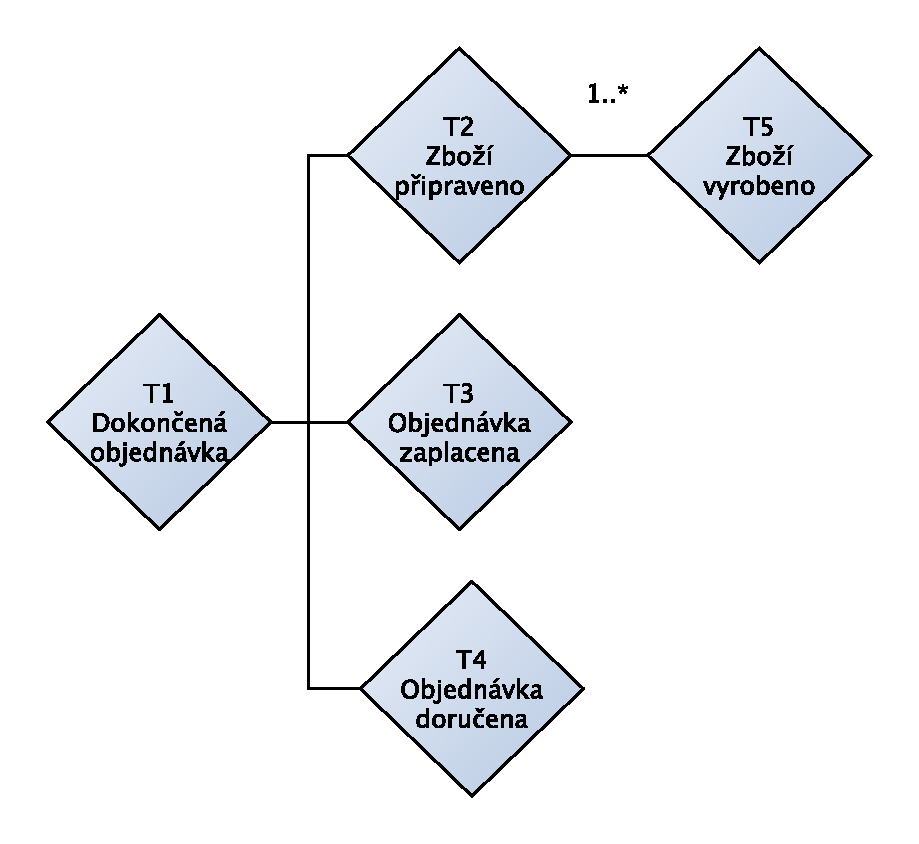
\includegraphics[width=1.0\textwidth]{obrazky/result-structure-chart}
\caption{Struktura závislosti transakcí v podnikovém procesu}
\label{fig:result_structure_chart}
\end{figure}

\subsection{Krok 6: Vytvoření DEMO modelů}
Nyní již máme dostatek informací pro vytvoření dvou DEMO modelů, které budou sloužit jako pevný bod pro verifikaci výsledného BPMN modelu i pro diskusi s business uživateli v případě požadavků na úpravy. Důvodem proč k této diskusi využívat DEMO modely (zejména ATD) a ne přímo výsledný BPMN model je vysoká úroveň komplexnosti BPMN modelu, který znesnadňuje jeho porozumění business uživateli.

Tabulky s popisem transakcí, které vznikly v Kroku 4 je dostatečným podkladem pro vytvoření DEMO Actor-Transaction Diagramu (ATD) i DEMO Process Structure Diagramu (PSD). ATD model zachycuje jevy v organizaci na nejvyšší úrovni abstrakce, tedy pouze actory a mezi nimi probíhající transakce. PSD jde o úroveň níže a zobrazuje jednotlivé transakční kroky stejně jako vzájemnou provázanost transakcí, kterou jsme indetifikovali v předchozím kroku. Oba modely jsou podrobně popsány v rámci kapitoly 4.

\subsection{Krok 7: Vytvoření BPMN modelu}
Nyní již máme vytvořený dostatečně silný základ a můžeme přikročit k vytvoření samotného BPMN modelu, který je výsledkem celé metody. Při jeho tvorbě využijeme zejména PSD diagram vytvořený v předchozím kroku a způsob vyjádření standardního transakčního vzoru pomocí \textit{úloh} a \textit{signálů} popsaný v sekci \ref{sec:tr_vzor_ulohy_signaly}.

Při vytváření BPMN modelu postupejeme tak, že následujeme PSD diagram od místa, kde dojde k provedení C-actu \textit{request} u kořenové transakce celého podnikového procesu a postupně převádíme jednotlivé transakční kroky do BPMN primitiv (\textit{úloh, signálů, sekvenčních toků, bran}) popsaných v sekci \ref{sec:tr_vzor_ulohy_signaly}. V případě, že je podnikový proces složen z více vzájemně provázaných transakcí musíme při vytváření BPMN modelu v momentě, kdy v PSD diagramu dojdeme na místo, kde je při provedení C-actu \textit{promise} vytvořen \textit{request} na další transakci, odklonit sekvenční tok a pokračovat v provádění transakčního vzoru transakce-potomka. Stejně tak pokračujeme i v dalších případech dokud se opět \uv{nevynoříme} (v případě, že všechny transakce-potomci dopadnou úspěšně) v kořenové transakci a jsme schopni provést exekuci P-actu.

%V případě potřeby a pokud máme identifikované reálné aktivity příslušné k jednotlivým transakčním krokům tak můžeme tyto kroky přejmenovat i v našem výsledném BPMN modelu.

\section{Další výzkum}

Obsah této práce je prvním pokusem o vytvoření metody pro vytváření BPMN modelů podnikových procesů za použití teoretických konstruktů z \ptheory, Enterprise ontology a metodologie DEMO. Jako každá první verze i tato musí být doplněna dalším výzkumem a všechna představená východiska musí být prověřena a potvrzena. Pro zdůraznění je zde vypsáno několik bodů, kde autor považuje další výzkum za nezbytný:

\begin{enumerate}
\item Posouzení důležitosti a případně vytvoření určité formy textového modelu na způsob DEMO Action Modelu, který umožní jednak naprosto přesně zachytit informace o agendě actorů v daném momentě, jednak bude sloužit jako podklad pro implementaci simulace modelu pomocí nějakého softwarového nástroje a jednak umožní formální verifikaci pomocí gramatiky, která bude pro takový model vytvořena.
\item Posouzení, zda je BPMN element \textit{úloha} dostatečný pro vyjádření DEMO C-actů a P-actů.
\item Posouzení použití konkrétních názvů aktivit pro jednotlivé transkační kroky indetifikované v Kroku 4 metody.
\item V DEMO verze 3 byla přidána do transakčního vzoru další vrstva umožňující prakticky kdykoliv \uv{vzít zpět} již vyjádřený C-act. Dalším výzkumem musí být posuzeno zda je toto možné znázornit v DEMO, jestli je to žádoucí a jaký to bude mít vliv na komplexnost výsledných BPMN modelů.
\item Návrh implementace automatického generování BPMN modelů z DEMO modelů pomocí vyjádření transakčního vzoru v BPMN dle sekce \ref{sec:vyjadreni_trans_vzor}. Výsledkem by mělo být propojení se softwarovou aplikací, kterou připravuje firma Formetis.
\end{enumerate}

\nocite{*}
\bibliographystyle{plain}
\bibliography{Bibliography}

\end{document}
